\documentclass[11pt,a4paper]{article}

% --------------------------------------------------
% PACKAGES
% --------------------------------------------------
\usepackage[utf8]{inputenc}
\usepackage[T1]{fontenc}
% babel[french] non disponible sur ce système — définitions manuelles
\newcommand{\og}{%
  \ifmmode\langle\else\guillemotleft\nobreak\fi}
\newcommand{\fg}{%
  \ifmmode\rangle\else\nobreak\guillemotright\fi}
\renewcommand{\today}{%
    \number\day\space
    \ifcase\month\or
    janvier\or f\'evrier\or mars\or avril\or mai\or juin\or
    juillet\or ao\^ut\or septembre\or octobre\or novembre\or d\'ecembre\fi
    \space\number\year
}
\usepackage{lmodern}
\usepackage{geometry}
\usepackage{amsmath,amssymb,amsthm}
\usepackage{array}
\usepackage{booktabs}
\usepackage{graphicx}
\graphicspath{{./}{../../}}
\usepackage{float}
\usepackage{hyperref}
\usepackage{xcolor}
\usepackage{enumitem}
\usepackage{listings}
\usepackage{fancyhdr}
\usepackage{titlesec}
\usepackage{caption}

\geometry{margin=2.5cm}
\setlength{\headheight}{14pt}
\setlength{\parskip}{0.5em}
\setlength{\parindent}{0pt}

% --------------------------------------------------
% HYPERREF
% --------------------------------------------------
\hypersetup{
    colorlinks=true,
    linkcolor=blue!60!black,
    urlcolor=blue!60!black,
    citecolor=blue!60!black,
    pdftitle={Projet Optimisation Discrète - VRPTW},
    pdfauthor={El Bouazzaoui Ali - Nadir Ayoub}
}

% --------------------------------------------------
% CODE STYLE
% --------------------------------------------------
\lstset{
    basicstyle=\ttfamily\small,
    breaklines=true,
    frame=single,
    columns=fullflexible,
    keepspaces=true
}

% --------------------------------------------------
% HEADER / FOOTER
% --------------------------------------------------
\pagestyle{fancy}
\fancyhf{}
\fancyhead[L]{Projet Optimisation Discrète}
\fancyhead[R]{VRPTW}
\fancyfoot[C]{\thepage}

% --------------------------------------------------
% TITLE FORMAT
% --------------------------------------------------
\titleformat{\section}{\large\bfseries}{\thesection.}{0.5em}{}
\titleformat{\subsection}{\normalsize\bfseries}{\thesubsection.}{0.5em}{}

% --------------------------------------------------
% DOCUMENT
% --------------------------------------------------
\begin{document}

\begin{titlepage}
    \centering
    {\scshape\LARGE Polytech Lyon \par}
    \vspace{1cm}
    {\scshape\Large Optimisation Discrète \par}
    \vspace{1.5cm}
    {\huge\bfseries Projet : Vehicle Routing Problem with Time Windows\par}
    \vspace{1.5cm}
    {\Large Rapport de projet\par}
    \vspace{2cm}
    
    \begin{tabular}{rl}
        Étudiants : & El Bouazzaoui Ali \\
                    & Nadir Ayoub \\
        Enseignant : & Stéphane Bonnevay \\
        Date : & 4 mai 2026
    \end{tabular}
    
    \vfill
    
    \begin{minipage}{0.9\textwidth}
    \small
    Ce rapport présente notre travail sur la résolution du problème de tournées de véhicules avec fenêtres de temps (VRPTW) à l'aide de métaheuristiques. Le sujet demande de modéliser le problème, de structurer le code, de déterminer le nombre minimal de véhicules, de générer des solutions aléatoires, puis d'implémenter et comparer deux métaheuristiques.
    \end{minipage}
    
    \vfill
\end{titlepage}

\tableofcontents
\newpage

% --------------------------------------------------
\section{Introduction}
% --------------------------------------------------

Le projet étudié porte sur le \textbf{Vehicle Routing Problem with Time Windows (VRPTW)}. L'objectif est de déterminer un ensemble de tournées partant et revenant au dépôt, de manière à desservir chaque client exactement une fois, en respectant les contraintes du problème et en minimisant la distance totale parcourue.

Le sujet demande explicitement :
\begin{itemize}
    \item de modéliser le problème et de structurer le code ;
    \item de déterminer, pour chaque jeu de données, le nombre minimum de véhicules ;
    \item de créer un générateur aléatoire de solutions ;
    \item d'implémenter deux métaheuristiques ;
    \item de comparer les résultats obtenus ;
    \item de commencer sans tenir compte des fenêtres de temps, puis de les ajouter ensuite.
\end{itemize}

Nous considérons d'abord le problème \textbf{sans fenêtres temporelles}, ce qui revient à traiter un \textbf{Capacitated Vehicle Routing Problem (CVRP)}. Les fenêtres de temps sont ensuite réintroduites pour traiter le problème complet.

% --------------------------------------------------
\section{Mode opératoire}
\label{sec:modeop}
% --------------------------------------------------

Cette section décrit comment reproduire nos expériences ou tester les algorithmes sur de nouvelles instances.

\subsection{Prérequis}

Le projet nécessite \textbf{Python 3.10} ou supérieur. Les dépendances pour l'affichage des figures sont installables avec :

\begin{lstlisting}
pip install matplotlib numpy
\end{lstlisting}

La résolution exacte (section bonus) nécessite en plus :

\begin{lstlisting}
pip install ortools
\end{lstlisting}

\subsection{Organisation des fichiers}

La structure du projet est la suivante :

\begin{lstlisting}
Projet_optimisation_El_Bouazzaoui_Ali-Nadir_Ayoub/
  data/                # instances .vrp a placer ici
    data101.vrp
    data102.vrp
    data111.vrp
    data112.vrp
    data201.vrp
    data202.vrp
    data1101.vrp
    data1102.vrp
    data1201.vrp
    data1202.vrp
  src/
    main.py              # point d'entree principal
    model.py             # structures de donnees
    io_utils.py          # lecture des fichiers .vrp
    evaluate.py          # calcul distances et faisabilite
    construction.py      # construction de solutions initiales
    neighbors.py         # operateurs de voisinage
    solver.py            # pilotage des experiences
    bonus_exact.py       # resolution exacte (OR-Tools)
    meta/
      simulated_annealing.py
      tabu_search.py
  rapport.pdf
\end{lstlisting}

Les fichiers d'instances \texttt{.vrp} doivent être placés dans un dossier \texttt{data/} à la racine du projet avant de lancer les commandes.

Toutes les commandes ci-dessous sont à lancer \textbf{depuis la racine du projet} (dossier \path{Projet_optimisation_El_Bouazzaoui_Ali-Nadir_Ayoub/}).

\subsection{Mode aperçu (défaut)}

La commande suivante affiche un résumé des instances, le premier nombre de véhicules faisable trouvé par notre construction en CVRP, des solutions aléatoires générées, et une première comparaison rapide des deux métaheuristiques. La recherche heuristique VRPTW n'est pas lancée par défaut dans ce mode, car elle est plus coûteuse ; les campagnes complètes sur les dix instances sont lancées avec le mode \texttt{experiment}.

\begin{lstlisting}
python src/main.py
\end{lstlisting}

\subsection{Mode expérimentation}

\paragraph{CVRP — preset rapide.}
Lance une campagne sur l'ensemble des instances sans fenêtres de temps, en quelques secondes :

\begin{lstlisting}
python src/main.py --mode experiment --preset quick
\end{lstlisting}

\paragraph{CVRP — preset long.}
Lance la campagne complète avec davantage d'itérations et cinq répétitions par instance (quelques minutes) :

\begin{lstlisting}
python src/main.py --mode experiment --preset long
\end{lstlisting}

\paragraph{VRPTW.}
L'option \texttt{--time-windows} active les fenêtres de temps :

\begin{lstlisting}
python src/main.py --mode experiment --preset long --time-windows
\end{lstlisting}

\paragraph{Instance unique avec détail run par run.}

\begin{lstlisting}
python src/main.py --mode experiment --preset quick \
    --instances data101.vrp --details
\end{lstlisting}

Les résultats sont enregistrés automatiquement dans \texttt{experiment\_results.log}. Un autre fichier peut être choisi avec \texttt{--output-file nom.log}.

\subsection{Mode bonus — résolution exacte}

Ce mode requiert OR-Tools. Il lance une résolution exacte sur des sous-instances de taille croissante extraites de \texttt{data101.vrp} :

\begin{lstlisting}
python src/main.py --mode bonus \
    --sizes 5 10 15 20 25 30 --time-limit 10
\end{lstlisting}

\subsection{Récapitulatif des options de \texttt{main.py}}

\begin{center}
\begin{tabular}{ll}
\toprule
Option & Description \\
\midrule
\texttt{--mode} & \texttt{overview} (défaut), \texttt{experiment}, \texttt{bonus} \\
\texttt{--preset} & \texttt{quick} ou \texttt{long} \\
\texttt{--instances} & fichiers \texttt{.vrp}, ex.\ \texttt{data101.vrp data202.vrp} \\
\texttt{--limit} & nombre maximal d'instances à traiter \\
\texttt{--time-windows} & active les contraintes temporelles (VRPTW) \\
\texttt{--method} & \texttt{both} (défaut), \texttt{sa} ou \texttt{tabu} \\
\texttt{--details} & affiche le détail par répétition \\
\texttt{--output-file} & fichier de sortie pour les résultats \\
\texttt{--sizes} & tailles des sous-instances (mode bonus) \\
\texttt{--time-limit} & limite de temps par sous-instance (mode bonus, en s) \\
\bottomrule
\end{tabular}
\end{center}

% --------------------------------------------------
\section{Organisation du projet}
% --------------------------------------------------

Afin de répondre progressivement aux différentes questions du sujet, nous avons découpé le travail en plusieurs phases.

\subsection{Phase 1 : Fondations du projet}
Cette phase regroupe :
\begin{itemize}
    \item la modélisation mathématique du problème ;
    \item la définition de la structure du code.
\end{itemize}

\subsection{Phase 2 : Détermination du nombre de véhicules}
Cette phase est décomposée en deux sous-parties :
\begin{itemize}
    \item sans fenêtres de temps ;
    \item avec fenêtres de temps.
\end{itemize}

\subsection{Phase 3 : Génération de solutions initiales}
La méthode retenue pour satisfaire la consigne de génération aléatoire consiste à construire des \textbf{solutions aléatoires faisables}.

\subsection{Phase 4 : Première métaheuristique}
Le \textbf{recuit simulé} est retenu comme première métaheuristique. Une première version fonctionnelle permet de valider la chaîne complète :
\begin{itemize}
    \item génération d'une solution initiale ;
    \item génération d'un voisin faisable ;
    \item acceptation déterministe ou probabiliste ;
    \item mémorisation de la meilleure solution rencontrée.
\end{itemize}

\subsection{Phase 5 : Deuxième métaheuristique}
La \textbf{recherche tabou} est retenue comme seconde métaheuristique. Une première version permet de disposer rapidement des deux approches demandées par le sujet avant de lancer les comparaisons expérimentales détaillées.

\subsection{Phase 6 : Protocole expérimental et comparaison}
L'infrastructure expérimentale distingue clairement deux usages :
\begin{itemize}
    \item le préréglage technique \texttt{quick}, utilisé comme \og mode rapide \fg{} pour valider les implémentations et obtenir un premier ordre de grandeur ;
    \item le préréglage technique \texttt{long}, utilisé comme \og mode long \fg{} pour les comparaisons plus rigoureuses, avec davantage d'itérations et plusieurs répétitions.
\end{itemize}

% --------------------------------------------------
\section{Modélisation du problème}
% --------------------------------------------------

\subsection{Description générale}
On considère un dépôt unique et un ensemble de clients. Chaque client possède :
\begin{itemize}
    \item des coordonnées cartésiennes ;
    \item une demande ;
    \item éventuellement une fenêtre de temps ;
    \item un temps de service.
\end{itemize}

Les véhicules sont supposés identiques et possèdent tous la même capacité maximale \(Q\).

L'objectif principal est de minimiser la distance totale parcourue. Le nombre de véhicules n'étant pas fixé dans le sujet, il doit être déterminé.

\subsection{Ensembles}
\[
V = \{0,1,\dots,n\}
\]
désigne l'ensemble des sommets, où :
\begin{itemize}
    \item \(0\) représente le dépôt ;
    \item \(C = \{1,\dots,n\}\) représente l'ensemble des clients.
\end{itemize}

\subsection{Paramètres}
\begin{itemize}
    \item \(d_{ij}\) : distance entre les sommets \(i\) et \(j\) ;
    \item \(q_i\) : demande du client \(i\) ;
    \item \(Q\) : capacité maximale d'un véhicule ;
    \item \(a_i\) : date de début de la fenêtre de temps du client \(i\) ;
    \item \(b_i\) : date de fin de la fenêtre de temps du client \(i\) ;
    \item \(s_i\) : durée de service chez le client \(i\).
\end{itemize}

\subsection{Variables de décision}
Une modélisation classique consiste à utiliser des variables binaires :
\[
x_{ij} =
\begin{cases}
1 & \text{si un véhicule va directement de } i \text{ vers } j, \\
0 & \text{sinon.}
\end{cases}
\]
avec
\[
x_{ij} \in \{0,1\} \qquad \forall i,j \in V,\ i \neq j.
\]

Pour la version avec fenêtres de temps, on introduit également :
\[
t_i = \text{instant de début de service au client } i.
\]
avec
\[
t_i \ge 0 \qquad \forall i \in V.
\]

\subsection{Fonction objectif}
L'objectif est de minimiser la distance totale parcourue :
\[
\min \sum_{i \in V} \sum_{j \in V,\, j \neq i} d_{ij} x_{ij}.
\]

\subsection{Contraintes principales}

\subsubsection{Visite unique de chaque client}
Chaque client doit être visité exactement une fois :
\[
\sum_{j \in V,\, j \neq i} x_{ij} = 1 \qquad \forall i \in C
\]
\[
\sum_{i \in V,\, i \neq j} x_{ij} = 1 \qquad \forall j \in C
\]

\subsubsection{Conservation du flot}
Si un véhicule arrive chez un client, il doit également en repartir :
\[
\sum_{j \in V} x_{ij} = \sum_{j \in V} x_{ji} \qquad \forall i \in C
\]

\subsubsection{Capacité}
Pour chaque véhicule, la somme des demandes des clients affectés à sa tournée ne doit pas dépasser \(Q\).

Dans une formulation compacte complète, cette contrainte s'écrit au moyen de variables supplémentaires d'affectation ou de charge. La formulation exacte en tournées n'est pas détaillée ici ; dans notre implémentation, la capacité est contrôlée lors de l'évaluation de chaque route.

\subsubsection{Fenêtres de temps}
Dans la seconde partie du projet, on ajoute :
\[
a_i \le t_i \le b_i
\]
et, dans une formulation PLNE classique, pour tout arc \((i,j)\) potentiellement utilisé,
\[
t_j \ge t_i + s_i + d_{ij} - M(1-x_{ij}) \qquad \forall i \neq j,
\]
où \(M\) est une constante suffisamment grande. Cette écriture précise que la contrainte d'enchaînement temporel n'est active que lorsque l'arc \((i,j)\) est effectivement utilisé. Dans notre implémentation, la faisabilité temporelle est ensuite contrôlée directement au niveau de l'évaluation de route.

Cette formulation correspond à un problème combinatoire NP-difficile, ce qui justifie le recours à des méthodes heuristiques et métaheuristiques pour traiter des instances de grande taille dans des temps de calcul raisonnables.

Une formulation complète du VRPTW peut être donnée sous forme de programme linéaire en nombres entiers. Dans ce cadre, des contraintes supplémentaires, par exemple de type MTZ ou de flot, peuvent être introduites pour éliminer les sous-tournées. Dans notre approche, nous n'implémentons pas explicitement ces contraintes, car la résolution repose sur des méthodes heuristiques qui construisent et améliorent directement des solutions faisables.

\subsection{Remarque sur l'utilisation d'OR-Tools}
Nous avons choisi d'utiliser OR-Tools uniquement pour des \textbf{tests sur petites instances} et pour la validation de certaines hypothèses. En effet, sur des instances plus grandes, l'utilisation directe d'un solveur exact peut devenir trop coûteuse en temps de calcul. La résolution principale du projet repose donc sur des méthodes heuristiques et métaheuristiques.

% --------------------------------------------------
\section{Structure du code}
% --------------------------------------------------

La structure du code a été pensée de manière modulaire, afin de séparer clairement les rôles de chaque composant. L'arborescence complète est présentée dans la section~\ref{sec:modeop}.

\subsection{Évolution de l'architecture}
La structure retenue est guidée par un principe simple : séparer clairement la lecture des données, l'évaluation des solutions, la construction initiale, la génération des voisinages, les métaheuristiques et le pilotage expérimental.

Le module \texttt{io\_utils.py} isole le parsing des fichiers \texttt{.vrp}. Le module \texttt{evaluate.py} centralise les calculs de distance, de charge et de faisabilité, de sorte que toutes les méthodes reposent sur la même définition d'une solution valide. Les autres modules séparent plus explicitement :
\begin{itemize}
    \item la construction des solutions ;
    \item l'évaluation des solutions ;
    \item la génération des voisins ;
    \item la logique propre à chaque métaheuristique ;
    \item le pilotage global des expériences.
\end{itemize}

Cette évolution n'est donc pas purement esthétique. Elle répond à un besoin de lisibilité, de réutilisation du code et de réduction des erreurs.

\subsection{Justification des choix de fichiers}
Le découpage en fichiers a été pensé pour suivre les grandes responsabilités du projet.

\begin{itemize}
    \item \texttt{io\_utils.py} regroupe tout ce qui concerne la lecture des données. Nous avons préféré isoler cette partie, car elle dépend fortement du format des fichiers et ne doit pas polluer la logique des algorithmes.
    \item \texttt{model.py} regroupe les structures de données du problème et facilite la circulation d'objets cohérents entre les modules ;
    \item \texttt{evaluate.py} joue le rôle de noyau commun et rassemble les calculs de distance, de charge et de faisabilité ;
    \item \texttt{construction.py} contient les méthodes de construction de solutions. Nous avons fait ce choix pour distinguer clairement les solutions initiales des méthodes d'amélioration.
    \item \texttt{neighbors.py} rassemble les transformations locales des solutions. Il nous a semblé plus propre d'avoir un module dédié aux mouvements, plutôt que de disperser ces opérations dans chaque métaheuristique.
    \item le dossier \texttt{meta/} contient les métaheuristiques elles-mêmes ; cette séparation facilite la comparaison des approches, car chaque méthode dispose de son propre fichier, avec ses paramètres et sa logique ;
    \item \texttt{solver.py} centralise le lancement des expériences, les préréglages et les synthèses statistiques ;
    \item \texttt{main.py} reste volontairement léger : son rôle est de lancer les traitements et d'afficher des synthèses, pas de contenir toute l'intelligence du projet.
\end{itemize}

\subsection{Justification du découpage modulaire}
La structure retenue fait évoluer l'architecture uniquement lorsque le besoin se présente concrètement : tant qu'un seul algorithme partageait peu de briques, un découpage fin n'était pas nécessaire ; dès que plusieurs algorithmes ont commencé à réutiliser les mêmes fonctions d'évaluation et de voisinage, la séparation est devenue naturelle. Cette approche permet à chaque fichier de correspondre à un rôle précis — construction, évaluation, voisinage, métaheuristique, pilotage — ce qui facilite à la fois les tests et la lecture du code.

\subsection{\texttt{main.py}}
Point d'entrée unique du programme. Il expose trois modes d'exécution via des arguments en ligne de commande :
\begin{itemize}
    \item \textbf{overview} (défaut) : affiche le résumé des instances, la recherche du premier nombre de véhicules faisable trouvé en CVRP, la génération de solutions aléatoires, et une première comparaison des métaheuristiques. Avec \texttt{--time-windows}, il affiche aussi la recherche heuristique VRPTW sur les instances sélectionnées ;
    \item \textbf{experiment} : lance une campagne structurée, avec choix du préréglage (\texttt{quick} ou \texttt{long}), de la méthode (\texttt{sa}, \texttt{tabu} ou \texttt{both}), du mode CVRP ou VRPTW, et des instances cibles ;
    \item \textbf{bonus} : applique un solveur exact (OR-Tools) à des sous-instances de taille croissante pour identifier le seuil de difficulté calculatoire.
\end{itemize}

\subsection{\texttt{model.py}}
Définit les trois structures de données fondamentales du projet sous forme de \textit{dataclasses} Python :
\begin{itemize}
    \item \texttt{Depot} : coordonnées \((x,y)\) et fenêtre de temps du dépôt ;
    \item \texttt{Client} : coordonnées, fenêtre de temps \([a_i, b_i]\), demande \(q_i\) et durée de service \(s_i\) ;
    \item \texttt{VRPTWInstance} : agrégat complet d'une instance (dépôt, dictionnaire de clients indexés, capacité maximale \(Q\)).
\end{itemize}
Ces structures sont importées par tous les autres modules, assurant une représentation uniforme des données dans l'ensemble du projet.

\subsection{\texttt{io\_utils.py}}
Parse les fichiers texte au format \texttt{.vrp} et retourne un objet \texttt{VRPTWInstance}. Il lit séquentiellement les métadonnées (nom, type, nombre de clients, capacité), les données du dépôt, puis celles de chaque client, et vérifie la cohérence entre le nombre de clients déclaré et le nombre effectivement lu.

\subsection{\texttt{evaluate.py}}
Noyau de calcul partagé par tous les modules. Pour une tournée donnée, il calcule :
\begin{itemize}
    \item la distance totale euclidienne, avec un cache des distances précalculées pour éviter les recalculs ;
    \item le profil temporel complet : temps d'arrivée, attente éventuelle, début et fin de service à chaque client, temps de retour au dépôt ;
    \item la faisabilité en capacité et la faisabilité temporelle, évaluées séparément.
\end{itemize}
Ce module joue un rôle central : toutes les décisions d'acceptation ou de rejet d'une solution — construction, voisinage, métaheuristiques — passent exclusivement par ses fonctions.

\subsection{\texttt{construction.py}}
Fournit les heuristiques de construction des solutions initiales. Deux stratégies sont implémentées :
\begin{itemize}
    \item une construction \textbf{déterministe par insertion faisable} : insère les clients un par un à la meilleure position admissible ; utilisée comme filet de sécurité sur les instances VRPTW fortement contraintes ;
    \item une construction \textbf{aléatoire randomisée} : choisit parmi les insertions les moins coûteuses, produisant des solutions variées pour favoriser la diversité des points de départ.
\end{itemize}
Ce module inclut également la fonction \texttt{find\_first\_feasible\_vehicle\_count}, qui incrémente \(k\) depuis la borne inférieure capacitaire jusqu'à trouver un nombre de véhicules faisable avec notre construction. L'ancien nom \texttt{find\_minimum\_vehicles} est conservé comme alias de compatibilité, mais le résultat doit être interprété avec prudence : il certifie le minimum seulement lorsqu'une solution CVRP est trouvée à la borne capacitaire \(LB\).

\subsection{\texttt{neighbors.py}}
Implémente les cinq opérateurs de voisinage utilisés par les deux métaheuristiques :
\begin{itemize}
    \item \texttt{relocate} : déplace un client vers une autre position, éventuellement dans une autre tournée ; les routes devenues vides sont supprimées automatiquement, permettant de réduire le nombre de véhicules en cours d'optimisation ;
    \item \texttt{swap} : échange deux clients entre eux, quelle que soit leur tournée d'origine ;
    \item \texttt{2-opt} : inverse un segment à l'intérieur d'une même tournée, supprimant les croisements locaux ;
    \item \texttt{or\_opt2} : déplace une paire de clients consécutifs vers une autre position dans la même tournée ou dans une autre, couvrant des restructurations que \texttt{relocate} ne peut pas atteindre ;
    \item \texttt{2-opt$^*$} : échange les suffixes de deux tournées distinctes, permettant des réorganisations globales entre routes.
\end{itemize}
Chaque candidat est validé par \texttt{evaluate.py} avant d'être retenu, garantissant que seules des solutions faisables sont proposées aux métaheuristiques.

\subsection{\texttt{solver.py}}
Orchestre les campagnes expérimentales. Il définit les deux préréglages (\texttt{quick} et \texttt{long}) comme structures immuables, lance les répétitions avec des graines déterministes, collecte les statistiques (moyenne, min, max) sur les distances et les temps d'exécution, et écrit les résultats dans un fichier de log. Il expose également les fonctions de formatage des tableaux récapitulatifs affichés en fin de campagne.

\subsection{\texttt{meta/simulated\_annealing.py}}
Implémente le recuit simulé. À chaque itération, un voisin faisable est tiré aléatoirement via l'un des cinq opérateurs de voisinage. Il est accepté systématiquement s'il améliore la solution courante, ou avec probabilité $\exp(-\Delta/T)$ sinon — où $T$ décroît géométriquement à chaque itération selon le facteur de refroidissement. La meilleure solution rencontrée est mémorisée tout au long de la recherche, indépendamment de la solution courante.

\subsection{\texttt{meta/tabu\_search.py}}
Implémente la recherche tabou. À chaque itération, un ensemble de voisins est échantillonné aléatoirement, puis le meilleur candidat non tabou est sélectionné. La mémoire tabou est une liste FIFO de signatures de solutions récemment visitées, de taille \textit{tenure}. Un critère d'aspiration permet d'accepter une solution tabou si elle améliore le meilleur résultat global connu.

\subsection{\texttt{bonus\_exact.py}}
Construit et résout des sous-instances de taille croissante via OR-Tools (solveur SCIP). Pour chaque taille \(n\), les \(n\) premiers clients de l'instance source sont extraits, le CVRP correspondant est modélisé en programme linéaire en nombres entiers, et soumis au solveur avec une limite de temps configurable. Les résultats indiquent le statut (optimal, réalisable ou infaisable) et l'objectif atteint.

% --------------------------------------------------
\section{Détermination du nombre de véhicules}
\label{sec:det_vehicules}
% --------------------------------------------------

\subsection{Principe général}
Le sujet demande de déterminer, pour chaque jeu de données, le nombre minimum de véhicules à utiliser. Nous distinguons ici deux niveaux de certitude : en CVRP, lorsqu'une solution faisable est trouvée avec \(k=LB\), la borne capacitaire prouve que ce nombre est minimal ; en VRPTW, nous reportons le plus petit \(k\) trouvé par notre procédure de construction, sans preuve exacte d'infaisabilité pour les valeurs plus petites.

Cette question est traitée en deux temps :
\begin{itemize}
    \item d'abord sans fenêtres de temps ;
    \item ensuite avec fenêtres de temps.
\end{itemize}

Dans cette première étape, nous ne considérons donc que :
\begin{itemize}
    \item la capacité des véhicules ;
    \item la nécessité de construire de vraies tournées partant et revenant au dépôt ;
    \item la distance entre les clients et le dépôt.
\end{itemize}

Autrement dit, nous traitons d'abord une version de type \textbf{CVRP} avant d'ajouter les fenêtres de temps.

\subsection{Borne inférieure théorique}
Une borne inférieure immédiate du nombre de véhicules est obtenue à partir de la somme des demandes :
\[
LB = \left\lceil \frac{\sum_{i \in C} q_i}{Q} \right\rceil.
\]

Cette borne est nécessaire mais pas toujours suffisante, car elle ne tient compte que de la capacité totale disponible. Elle ignore :
\begin{itemize}
    \item la répartition des demandes entre les tournées ;
    \item la structure géographique des clients ;
    \item la cohérence réelle des trajets.
\end{itemize}

Deux clients compatibles en termes de charge peuvent en effet être très éloignés, ce qui rend leur regroupement peu pertinent dans une même tournée.

\subsection{Choix méthodologique}
Nous avons décidé de ne pas nous limiter au calcul de la borne de capacité : il faut aussi construire effectivement des tournées faisables avec ce nombre de véhicules.

Notre méthode consiste donc à :
\begin{enumerate}[label=\arabic*.]
    \item calculer la borne inférieure \(LB\) ;
    \item fixer \(k = LB\) ;
    \item essayer de construire une solution faisable avec exactement \(k\) véhicules ;
    \item si aucun ensemble de tournées faisables n'est obtenu, incrémenter \(k\) ;
    \item retenir le premier \(k\) pour lequel tous les clients sont servis.
\end{enumerate}

Cette estimation doit être lue comme un résultat expérimental obtenu à l'aide d'une procédure de construction heuristique. Dans notre code final, la recherche du plus petit \(k\) repose sur une construction systématique faisable plutôt que sur un unique tirage aléatoire, ce qui limite la variabilité de cette étape. En CVRP, lorsqu'elle atteint \(LB\), la minimalité est certifiée par la borne de capacité ; en VRPTW, le résultat reste heuristique.

\subsection{Heuristique utilisée pour tester une valeur de \(k\)}
Pour tester si \(k\) véhicules suffisent, nous utilisons une heuristique gloutonne géographique sous contrainte de capacité.

Le principe est le suivant :
\begin{enumerate}[label=\arabic*.]
    \item initialiser \(k\) tournées vides ;
    \item choisir un premier client pour chaque tournée ;
    \item compléter chaque tournée en ajoutant à chaque étape un client non encore servi ;
    \item parmi les clients admissibles, sélectionner celui qui minimise la distance au dernier client de la tournée ;
    \item ne jamais dépasser la capacité maximale \(Q\) ;
    \item s'arrêter lorsque plus aucun client ne peut être ajouté à la tournée courante.
\end{enumerate}

Un client est dit \textbf{admissible} si son ajout à la tournée ne fait pas dépasser la capacité du véhicule.

\subsection{Critère de faisabilité}
Pour une valeur donnée de \(k\), la solution est considérée comme faisable si :
\begin{itemize}
    \item tous les clients sont affectés à une unique tournée ;
    \item la charge de chaque tournée est inférieure ou égale à \(Q\).
\end{itemize}

Dans cette phase, la distance intervient comme \textbf{critère de construction} des tournées, mais pas encore comme objectif d'optimisation final.

Du point de vue de l'implémentation, cette vérification est maintenant centralisée dans le module \texttt{evaluate.py}. Cela permet d'éviter la duplication des contrôles et garantit que les futures méthodes de construction et d'amélioration utiliseront toutes le même critère de faisabilité.

\subsection{Remarque}
Cette approche fournit une estimation cohérente du nombre de véhicules à utiliser. Elle devient une preuve de minimalité uniquement dans le cas CVRP lorsque le nombre trouvé est égal à la borne inférieure \(LB\). Pour le VRPTW, elle ne prouve pas qu'aucune autre construction ne pourrait réussir avec moins de véhicules.

\subsection{Résultats obtenus sans fenêtres de temps}
Nous avons appliqué notre méthode de construction gloutonne géographique à l'ensemble des instances, en partant à chaque fois de la borne inférieure $LB$ définie à la section précédente.

Pour chaque instance testée, notre procédure heuristique a trouvé une solution faisable dès la borne $LB$, sans avoir à incrémenter $k$. Il s'agit d'un résultat expérimental propre au corpus étudié : rien ne garantit que cette coïncidence se reproduirait sur d'autres instances.

\begin{center}
\begin{tabular}{lcccc}
\toprule
Instance & Capacité & Demande totale & \(LB\) & Nombre trouvé \\
\midrule
data101.vrp  & 200  & 1458 & 8 & 8 \\
data102.vrp  & 200  & 1458 & 8 & 8 \\
data1101.vrp & 200  & 1724 & 9 & 9 \\
data1102.vrp & 200  & 1724 & 9 & 9 \\
data111.vrp  & 200  & 1458 & 8 & 8 \\
data112.vrp  & 200  & 1458 & 8 & 8 \\
data1201.vrp & 1000 & 1724 & 2 & 2 \\
data1202.vrp & 1000 & 1724 & 2 & 2 \\
data201.vrp  & 1000 & 1458 & 2 & 2 \\
data202.vrp  & 1000 & 1458 & 2 & 2 \\
\bottomrule
\end{tabular}
\end{center}

Sur ce corpus, notre procédure heuristique a donc trouvé une solution faisable dès $LB$ pour chaque instance. Comme aucun nombre de véhicules strictement inférieur à \(LB\) ne peut transporter toute la demande, ces valeurs sont bien minimales pour la version CVRP de ces instances. La contrainte de capacité seule semble donc déterminante ici ; ce constat ne garantit pas que la même situation se reproduirait sur d'autres corpus.

\subsection{Influence des fenêtres de temps sur la borne inférieure}

La borne $LB$ ne dépend que de la demande totale et de la capacité $Q$ ; elle est donc indépendante des distances et des fenêtres temporelles. En revanche, les fenêtres de temps restreignent fortement l'ensemble des tournées faisables : deux clients compatibles en capacité peuvent être incompatibles temporellement et ne pas pouvoir être servis dans la même tournée. Cette contrainte peut donc augmenter le nombre de véhicules nécessaires :

\[
k_{TW} \ge LB.
\]

L'objectif de cette section est donc de déterminer expérimentalement $k_{TW}$ pour chaque instance, c'est-à-dire le premier nombre de véhicules pour lequel notre construction par insertion trouve une solution temporellement faisable.

\begin{center}
\begin{tabular}{lccc}
\toprule
Instance & \(LB\) capacité & \(k\) CVRP certifié & \(k\) VRPTW trouvé \\
\midrule
data101.vrp  & 8 & 8 & 21 \\
data102.vrp  & 8 & 8 & 18 \\
data1101.vrp & 9 & 9 & 18 \\
data1102.vrp & 9 & 9 & 16 \\
data111.vrp  & 8 & 8 & 14 \\
data112.vrp  & 8 & 8 & 12 \\
data1201.vrp & 2 & 2 & 5 \\
data1202.vrp & 2 & 2 & 4 \\
data201.vrp  & 2 & 2 & 5 \\
data202.vrp  & 2 & 2 & 5 \\
\bottomrule
\end{tabular}
\end{center}

\begin{figure}[H]
    \centering
    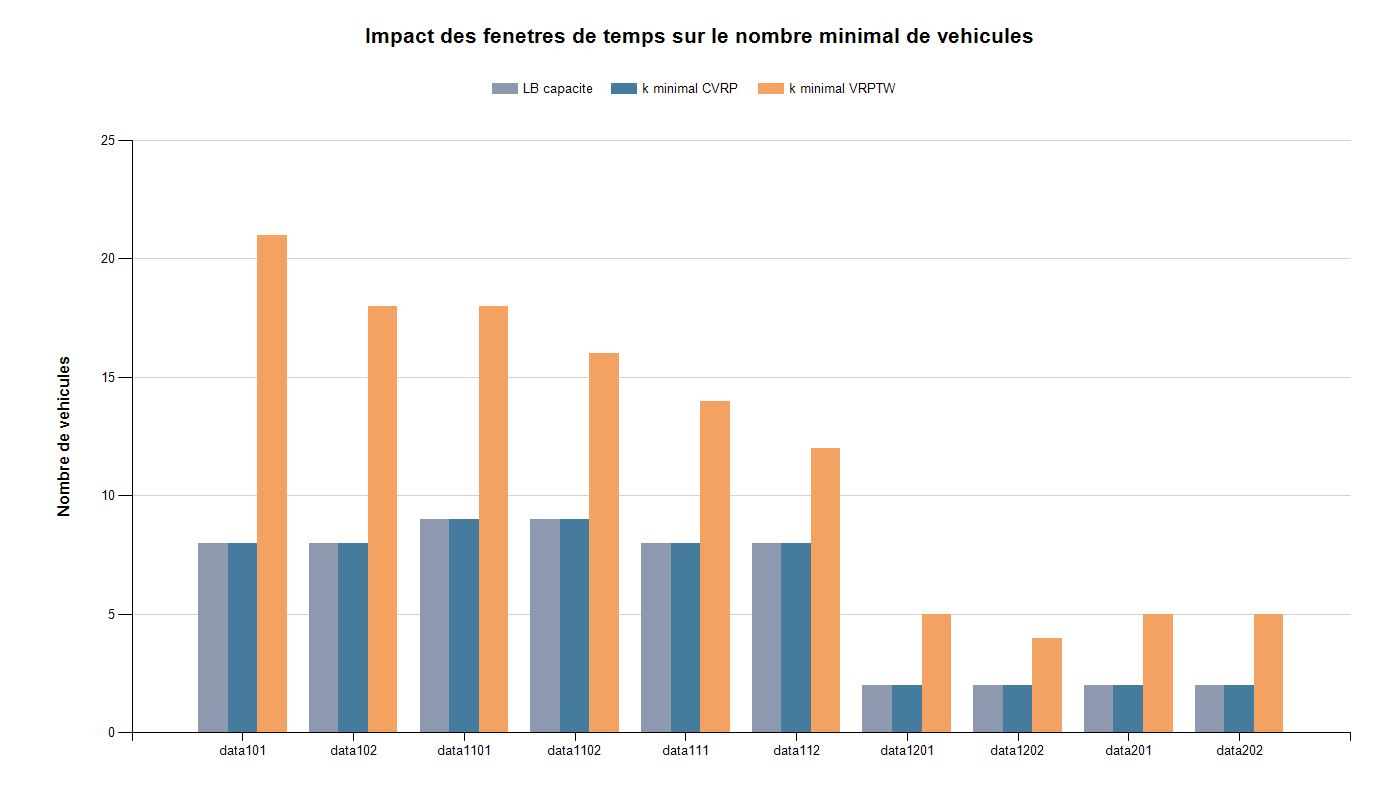
\includegraphics[width=\textwidth]{figures/comparison_vehicles.png}
    \caption{Impact des fenêtres de temps sur le nombre de véhicules trouvé.}
\end{figure}

\subsection{Première intégration effective des fenêtres de temps}
Après avoir d'abord travaillé sur la version capacitaire, nous avons intégré explicitement les fenêtres de temps dans la construction des tournées. Le simple prolongement de l'heuristique gloutonne précédente ne suffisait pas, car ajouter systématiquement les clients en fin de tournée se révélait trop rigide dans le cas VRPTW.

Nous avons donc fait évoluer la construction vers une logique d'insertion faisable. L'idée est de partir d'un ensemble de tournées initialement vides, puis d'insérer progressivement les clients dans les positions qui restent compatibles avec :
\begin{itemize}
    \item la capacité du véhicule ;
    \item les fenêtres de temps ;
    \item le retour au dépôt dans la fenêtre autorisée.
\end{itemize}

Ce changement de stratégie est important du point de vue méthodologique : il illustre bien le fait qu'une structure de construction adaptée au CVRP ne se transpose pas automatiquement au VRPTW.

\subsection{Premiers résultats VRPTW}
Les premiers essais confirment que les fenêtres de temps modifient profondément la structure du problème : là où la version capacitaire permettait d'atteindre directement la borne $LB$, la version VRPTW exige un nombre de véhicules bien plus élevé, comme le montrent les résultats complets du tableau de la section précédente.

\subsection{Limites observées : générateur aléatoire VRPTW}
Cette première intégration des fenêtres de temps s'accompagne d'une limite importante. Le générateur aléatoire de solutions initiales, qui fonctionne correctement en CVRP, ne parvient pas à produire facilement des solutions faisables en VRPTW. Sur \texttt{data101.vrp} par exemple, le taux de succès est inférieur à $3\,\%$ : moins de $3$ tentatives sur $100$ aboutissent à une solution temporellement faisable.

En pratique, nous limitons le générateur à $3$ tentatives par run en mode VRPTW (pour éviter des temps de calcul prohibitifs). Quasiment toutes les répétitions démarrent donc de la \emph{même} solution initiale déterministe. Conséquence directe : la variabilité entre répétitions ne reflète pas une diversité de points de départ, mais uniquement les fluctuations stochastiques internes aux métaheuristiques. Les écarts-types observés en VRPTW mesurent donc la robustesse intra-run, et non une vraie diversité inter-runs.

Ce constat illustre qu'intégrer les fenêtres de temps ne se résume pas à activer un test de faisabilité supplémentaire : il faut aussi adapter les briques de construction.

\subsection{Première extension des métaheuristiques au cas VRPTW}
Malgré cette limite, nous avons pu commencer à étendre les métaheuristiques à la version avec fenêtres de temps en utilisant une solution initiale déterministe faisable comme point de départ.

Concrètement, lorsque la génération aléatoire échoue en mode VRPTW, nous utilisons la construction par insertion faisable pour fournir une solution initiale aux métaheuristiques. Cette stratégie n'est pas encore la version finale souhaitée, mais elle permet déjà de tester le comportement des algorithmes sur le vrai problème avec contraintes temporelles.

Un premier test ciblé a ainsi été réalisé sur l'instance \texttt{data1201.vrp}. Avec \(k=5\) véhicules, le recuit simulé a pu être exécuté à partir d'une solution initiale VRPTW faisable, tout en conservant la faisabilité de la solution au cours de l'optimisation.

Cette étape constitue une transition importante : même si l'initialisation aléatoire VRPTW reste à fiabiliser, la chaîne \og construction faisable + amélioration locale \fg{} devient déjà exploitable.

\subsection{Premier essai expérimental VRPTW}
Nous avons ensuite lancé un premier essai expérimental en mode rapide sur l'instance \texttt{data1201.vrp}, avec fenêtres de temps activées. La solution initiale faisable obtenue présente une distance de \(1974.63\).

Dans ce premier essai :
\begin{itemize}
    \item le recuit simulé améliore la solution et atteint une distance de \(1909.98\) ;
    \item la recherche tabou atteint une distance de \(1945.36\).
\end{itemize}

Les temps de calcul observés sont d'environ \(0.74\) seconde pour le recuit simulé et \(9.35\) secondes pour la recherche tabou.

Ce résultat reste préliminaire, mais il est important : il montre que nous disposons désormais d'une première chaîne expérimentale opérationnelle sur la vraie version VRPTW, même si elle repose encore sur une initialisation déterministe plutôt que sur un générateur aléatoire pleinement robuste.

Les campagnes expérimentales VRPTW (mode rapide et mode long) sont présentées dans la section~\ref{sec:metaheuristiques}, consacrée aux méthodes de résolution et aux résultats expérimentaux.

% --------------------------------------------------
\section{Génération d'une solution initiale}
% --------------------------------------------------

Le sujet demande explicitement la création d'un générateur aléatoire de solutions. La réponse retenue consiste à construire une \textbf{solution aléatoire faisable}.

\subsection{Choix retenu}
Nous ne retenons pas une permutation totalement aléatoire des clients, car celle-ci produit très souvent des solutions infaisables. À la place, nous construisons la solution progressivement :

\begin{enumerate}[label=\arabic*.]
    \item ouvrir une nouvelle tournée ;
    \item déterminer la liste des clients admissibles dans cette tournée ;
    \item choisir aléatoirement l'un de ces clients ;
    \item l'ajouter à la tournée ;
    \item recommencer jusqu'à ce qu'aucun autre client admissible ne puisse être ajouté ;
    \item ouvrir une nouvelle tournée ;
    \item répéter jusqu'à ce que tous les clients soient servis.
\end{enumerate}

Une génération totalement aléatoire des tournées conduit dans la grande majorité des cas à des solutions infaisables, en particulier lorsque les contraintes de capacité et de temps sont fortes. Nous avons donc retenu une génération aléatoire faisable, construite progressivement, afin de conserver de la diversité sans perdre le contrôle de la faisabilité.

Dans notre implémentation actuelle, nous fixons d'abord un nombre de tournées \(k\), en pratique le nombre de véhicules retenu dans la phase précédente. Nous initialisons ensuite ces \(k\) tournées puis nous ajoutons des clients un par un de manière aléatoire, sous réserve d'admissibilité.

À chaque étape, un client est considéré comme admissible si son ajout en fin de tournée conserve la faisabilité de cette tournée. Le choix final est ensuite effectué aléatoirement parmi l'ensemble des clients admissibles. Cette stratégie permet de produire des solutions variées tout en restant contrôlées.

\subsection{Cas sans fenêtres de temps}
Dans le cas CVRP, un client est admissible si son ajout ne fait pas dépasser la capacité du véhicule.

\subsection{Cas avec fenêtres de temps}
Dans le cas VRPTW, un client est admissible si son ajout respecte à la fois :
\begin{itemize}
    \item la capacité du véhicule ;
    \item la faisabilité temporelle de la tournée.
\end{itemize}

\subsection{Intérêt de cette construction}
Cette méthode présente deux avantages importants pour la suite du projet :
\begin{itemize}
    \item elle génère plusieurs solutions initiales différentes pour une même instance, ce qui est utile pour évaluer la robustesse des métaheuristiques ;
    \item elle s'appuie sur le même module d'évaluation que le reste du projet, ce qui garantit une cohérence entre construction, tests de faisabilité et futurs mouvements de voisinage.
\end{itemize}

\subsection{Rôle de cette solution}
Cette solution initiale n'a pas vocation à être optimale. Elle sert de point de départ aux métaheuristiques.

Le générateur aléatoire répond pleinement au besoin dans le cas capacitaire, mais reste moins robuste dans le cas VRPTW fortement contraint. Une construction faisable déterministe est alors utilisée comme mécanisme de secours. La consigne du sujet sur la génération aléatoire est donc bien couverte, tout en assumant clairement que la variante VRPTW demeure perfectible.

La robustesse du générateur peut être évaluée empiriquement à partir de sa capacité à produire rapidement une solution faisable. Dans le cas CVRP, les essais menés montrent que cette génération aléatoire faisable fonctionne très facilement. En revanche, dans le cas VRPTW, la proportion de solutions directement faisables diminue nettement en raison des contraintes temporelles plus restrictives. Pour pallier cette limite, nous combinons génération aléatoire et construction déterministe, ce qui permet de conserver à la fois diversité et faisabilité.

% --------------------------------------------------
\section{Choix des méthodes de résolution}
\label{sec:metaheuristiques}
% --------------------------------------------------

Le projet demande l'utilisation de deux métaheuristiques. Les approches retenues sont les suivantes :
\begin{itemize}
    \item le recuit simulé ;
    \item la recherche tabou.
\end{itemize}

Ces deux méthodes sont particulièrement adaptées à une résolution par voisinage du problème de tournées de véhicules.

\subsection{Implémentation du recuit simulé}
Le recuit simulé a été implémenté dans une première version pragmatique. L'idée est de partir d'une solution initiale faisable, puis de répéter les étapes suivantes :
\begin{enumerate}[label=\arabic*.]
    \item tirer un voisin faisable de manière aléatoire ;
    \item calculer la variation de coût associée ;
    \item accepter systématiquement un voisin meilleur ;
    \item accepter parfois un voisin moins bon avec une probabilité dépendant de la température ;
    \item diminuer progressivement la température ;
    \item conserver la meilleure solution rencontrée pendant toute l'exécution.
\end{enumerate}

Le recuit simulé présente ici un avantage important : il permet d'accepter temporairement certaines dégradations de la solution afin d'échapper aux minima locaux et d'explorer plus largement l'espace des solutions. Cette méthode présente ainsi l'avantage de concilier diversification et intensification avec un coût de calcul modéré.

Nous avons volontairement choisi, pour cette première version, de générer un voisin aléatoire faisable plutôt que d'énumérer tous les voisins à chaque itération. Ce choix réduit fortement le coût d'une itération et rend l'algorithme plus adapté aux tests répétés sur des instances de taille 100.

\subsection{Pseudo-code simplifié du recuit simulé}
Le principe de l'algorithme peut être résumé par le pseudo-code suivant :

\begin{lstlisting}
Initialiser une solution s
Initialiser la temperature T
Tant que la condition d'arret n'est pas atteinte :
    generer un voisin faisable s'
    calculer Delta = f(s') - f(s)
    si Delta < 0 :
        accepter s'
    sinon :
        accepter s' avec une probabilite exp(-Delta / T)
    mettre a jour la temperature
Retourner la meilleure solution trouvee
\end{lstlisting}

\subsection{Résultats préliminaires}
Les premiers essais montrent déjà que le recuit simulé améliore nettement les solutions initiales aléatoires. Par exemple, sur l'instance \texttt{data101.vrp}, un test de validation a permis de passer d'une distance initiale de \(3488.41\) à une meilleure distance de \(2211.87\) en \(500\) itérations, tout en conservant une solution faisable.

Ces résultats restent préliminaires. Ils servent à valider l'implémentation et à préparer les futurs tests expérimentaux plus longs, qui feront l'objet d'un protocole plus rigoureux dans la suite du projet.

\subsection{Première implémentation de la recherche tabou}
La recherche tabou a également été implémentée dans une première version opérationnelle. À chaque itération, l'algorithme génère un ensemble de voisins faisables, puis sélectionne le meilleur voisin autorisé, c'est-à-dire non tabou, sauf si un critère d'aspiration permet d'accepter une solution améliorant le meilleur résultat global.

Dans cette première version, la mémoire tabou porte sur les signatures des solutions récemment visitées. Cette approche n'est pas la plus fine possible, mais elle permet de disposer rapidement d'une base fiable pour les expériences comparatives.

La recherche tabou repose sur une mémoire à court terme des mouvements ou solutions récentes, ce qui permet d'éviter les cycles et de forcer l'exploration de nouvelles régions de l'espace des solutions. Cette propriété devient particulièrement utile lorsque l'espace faisable est fortement contraint.

\subsection{Observation importante sur le coût de calcul}
Les premiers essais montrent que la recherche tabou est sensiblement plus coûteuse en temps de calcul que le recuit simulé dans notre implémentation actuelle. Cette différence s'explique par le fait que, même avec une limitation du nombre de voisins inspectés, la recherche tabou évalue un ensemble de candidats à chaque itération alors que le recuit simulé peut se contenter d'un voisin aléatoire faisable.

Cette observation est importante pour la suite du projet. Elle signifie que les tests de validation rapide et les tests expérimentaux longs devront être distingués clairement, avec des paramètres adaptés à chaque usage.

\subsection{Résultats préliminaires de la recherche tabou}
Sur l'instance \texttt{data101.vrp}, un test ciblé a permis d'améliorer une solution initiale de distance \(3604.26\) vers une distance \(3278.86\) en \(10\) itérations. Un aperçu plus léger intégré au programme principal améliore également la solution initiale, mais avec un coût de calcul déjà notable même pour un très petit nombre d'itérations.

Ces résultats confirment que la méthode fonctionne, tout en montrant qu'une attention particulière devra être portée au réglage des paramètres et au protocole de test.

\subsection{Mise en place du protocole expérimental}
Afin d'éviter de mélanger validation fonctionnelle et comparaison scientifique, nous avons centralisé les expériences dans un module dédié. Ce module permet :
\begin{itemize}
    \item de fixer des jeux de paramètres reproductibles ;
    \item de lancer plusieurs répétitions avec des graines différentes ;
    \item de résumer les résultats sous forme de moyennes, minimums et maximums ;
    \item de comparer directement les distances finales et les temps de calcul des deux métaheuristiques.
\end{itemize}

Deux préréglages sont utilisés :
\begin{itemize}
    \item \texttt{quick}, pour les vérifications rapides ;
    \item \texttt{long}, pour les tests approfondis.
\end{itemize}

\subsection{Paramètres retenus}
Le tableau suivant synthétise les paramètres utilisés dans les deux préréglages expérimentaux.

\begin{center}
\begin{tabular}{lcc}
\toprule
Paramètre & \texttt{quick} & \texttt{long} \\
\midrule
Itérations recuit simulé & 300 & 3000 \\
Température initiale & 100.0 & 150.0 \\
Facteur de refroidissement & 0.98 & 0.997 \\
Tentatives de voisinage par itération (RS) & 50 & 100 \\
Itérations recherche tabou & 5 & 60 \\
Tenure tabou & 5 & 20 \\
Voisins max évalués par itération & 40 & 200 \\
Répétitions par instance & 1 & 5 \\
\bottomrule
\end{tabular}
\end{center}

\subsection{Analyse des opérateurs de voisinage}
\label{sec:operateurs}

Les cinq opérateurs ont des propriétés structurellement différentes qui expliquent en partie les performances observées.

\begin{center}
\begin{tabular}{llccl}
\toprule
Opérateur & Portée & \multicolumn{2}{c}{Taux de faisabilité} & Rôle principal \\
          &        & CVRP & VRPTW & \\
\midrule
\texttt{relocate}  & intra/inter & 55\,\% & 3\,\%  & Rééquilibrage des tournées \\
\texttt{swap}      & intra/inter & 74\,\% & 1\,\%  & Correction d'affectations \\
\texttt{2-opt}     & intra       &100\,\% & 0\,\%  & Suppression de croisements \\
\texttt{or-opt(2)} & intra/inter & 30\,\% & 1\,\%  & Déplacement de paires \\
\texttt{2-opt*}    & inter       & 17\,\% & 6\,\%  & Restructuration inter-tournées \\
\bottomrule
\end{tabular}
\end{center}

Les taux sont mesurés sur \texttt{data101.vrp} (500 tentatives par opérateur, une tentative par appel), à partir de solutions initiales représentatives du problème considéré ($k=8$ en CVRP, $k=21$ en VRPTW).

\textbf{En CVRP,} \texttt{2-opt} est toujours faisable ($100\,\%$) car l'inversion d'un segment intra-route ne modifie pas la charge totale, seule contrainte active. \texttt{swap} et \texttt{relocate} sont moins systématiquement faisables car ils peuvent déséquilibrer les charges. \texttt{2-opt*} a le taux le plus faible ($17\,\%$) : les échanges de suffixes entre tournées produisent souvent des routes dépassant la capacité.

\textbf{En VRPTW,} la situation est radicalement différente. \texttt{2-opt} tombe à $0\,\%$ : la solution initiale VRPTW est à la limite de faisabilité temporelle pour chaque tournée, et l'inversion d'un segment perturbe l'ordre de visite et viole quasi-systématiquement au moins une fenêtre de temps. \texttt{2-opt*} affiche paradoxalement le meilleur taux VRPTW ($6\,\%$) car l'échange de suffixes peut parfois associer des clients aux fenêtres compatibles entre deux tournées. La densité totale du voisinage est environ dix fois plus faible en VRPTW qu'en CVRP, ce qui explique directement le surcoût en temps des campagnes VRPTW.

\textbf{Lien avec la comparaison RS/tabou.} En CVRP, l'espace faisable est dense : le RS trouve un voisin en 1 à 2 tentatives et peut explorer largement en 3\,000 itérations. En VRPTW, la faible densité signifie que chaque tentative échoue la plupart du temps (jusqu'à 100 tentatives par opérateur configurées dans le preset \texttt{long}). La tabou, qui évalue plusieurs candidats par itération et garde le meilleur non tabou, tire mieux parti de cet espace restreint car elle ne gaspille pas son budget sur des directions aléatoires — c'est l'explication algorithmique fondamentale de sa supériorité en VRPTW.

\subsection{Étude de sensibilité aux paramètres}

Pour valider les choix de paramètres, nous avons isolé l'effet de chaque paramètre clé sur \texttt{data101.vrp} en CVRP (preset \texttt{long}, une répétition, graine fixe), en ne faisant varier qu'un paramètre à la fois.

\subsubsection*{Recuit simulé — température initiale \(T_0\)}

\begin{center}
\begin{tabular}{ccc}
\toprule
\(T_0\) & Meilleure distance & Commentaire \\
\midrule
50  & 1304.65 & Légèrement en retrait sur ce test \\
100 & 1202.07 & Meilleure valeur sur ce test \\
\textbf{150} & \textbf{1265.78} & \textbf{Valeur retenue — robustesse VRPTW} \\
200 & 1224.65 & Résultat proche de T0=100 \\
300 & 1379.81 & Trop de marche aléatoire initiale \\
\bottomrule
\end{tabular}
\end{center}

La plage $T_0 \in [50, 200]$ donne des résultats comparables sur ce test (écart inférieur à $9\,\%$) ; $T_0=300$ est clairement pénalisant. $T_0=100$ donne le meilleur résultat sur ce test à graine unique, mais $T_0=150$ a été retenu car il offre un taux d'acceptation des dégradations plus élevé en début de recherche, ce qui s'avère bénéfique en VRPTW où le voisinage faisable est très restreint et chaque mouvement dégradant accepté est plus coûteux à trouver.

\subsubsection*{Recuit simulé — facteur de refroidissement \(\alpha\)}

\begin{center}
\begin{tabular}{ccc}
\toprule
\(\alpha\) & Meilleure distance & Commentaire \\
\midrule
0.990 & 1680.37 & Temperature $< 1$ dès l'itération 460 \\
0.995 & 1506.11 & Convergence prématurée \\
\textbf{0.997} & \textbf{1265.78} & \textbf{Valeur retenue} \\
0.999 & 1935.99 & Temperature encore haute à la fin des 3\,000 itérations \\
\bottomrule
\end{tabular}
\end{center}

Ce paramètre est le plus sensible. Avec $\alpha=0.99$, la température tombe sous 1 dès l'itération~460, bloquant l'exploration pour les 2\,540 itérations restantes. Avec $\alpha=0.999$, la temperature atteindrait $T=1$ à l'itération~11\,500 : l'algorithme marche aléatoirement jusqu'au bout sans converger.

\subsubsection*{Recherche tabou — nombre maximal de voisins par itération}

\begin{center}
\begin{tabular}{ccc}
\toprule
\texttt{max\_neighbors} & Meilleure distance & Commentaire \\
\midrule
50  & 1643.60 & Voisinage trop réduit par itération \\
100 & 1450.49 & Intermédiaire \\
\textbf{200} & \textbf{1300.51} & \textbf{Valeur retenue} \\
400 & 1219.81 & Meilleure qualité mais temps $\times\,2$ \\
\bottomrule
\end{tabular}
\end{center}

C'est le paramètre le plus impactant pour la tabou : plus l'échantillon par itération est grand, meilleure est la solution, car la tabou dispose d'un choix plus représentatif du voisinage à chaque itération. La tenure ($5$, $10$, $20$, $30$) ne produit aucune différence sur cette instance (distance $= 1300.51$ dans les quatre cas), car l'espace des solutions sur 100 clients est suffisamment vaste pour que l'interdiction de quelques solutions récentes ne soit pas contraignante.

\subsection{Comparaison du nombre de solutions explorées}

\subsubsection*{Volume d'exploration par préréglage}

\begin{center}
\begin{tabular}{lccc}
\toprule
Méthode & Itérations & Évalué par itération & Total évalués \\
\midrule
RS — \texttt{quick}    & 300  & 1 & $\leq 300$ \\
RS — \texttt{long}     & 3000 & 1 & $\leq 3000$ \\
Tabou — \texttt{quick} & 5    & $\leq 40$ & $\leq 200$ \\
Tabou — \texttt{long}  & 60   & $\leq 200$ & $\leq 12\,000$ \\
\bottomrule
\end{tabular}
\end{center}

Le RS évalue exactement 1 voisin faisable par itération. La tabou en évalue jusqu'à \texttt{max\_neighbors} par itération, puis sélectionne le meilleur non tabou. En preset \texttt{long}, la tabou peut donc traiter 4 fois plus de candidats, ce qui justifie son coût en temps et sa meilleure qualité en VRPTW.

\subsubsection*{Profil d'acceptation du recuit simulé}

Sur \texttt{data101.vrp} en CVRP avec le preset \texttt{long} ($T_0=150$, $\alpha=0.997$, 3\,000 itérations) :
\begin{itemize}
    \item voisins faisables trouvés : 3\,000/3\,000 ($100\,\%$) ;
    \item mouvements améliorants acceptés : 512 ($17\,\%$) ;
    \item mouvements dégradants acceptés : 334 ($11\,\%$) ;
    \item total accepté : 846 ($28\,\%$).
\end{itemize}

Le RS accepte environ un mouvement dégradant pour 1,5 amélioration. Ce ratio de diversification est effectif et décroît naturellement au fil du refroidissement : en début de recherche, le taux d'acceptation des dégradations est voisin de $40\,\%$ ; il devient quasi-nul dans les dernières centaines d'itérations.

\subsubsection*{Effet du mode VRPTW sur la densité du voisinage}

En VRPTW, le taux de réussite moyen des opérateurs chute de $\sim 55\,\%$ (CVRP) à $\sim 4\,\%$ (VRPTW). Le RS nécessite en moyenne 25 tentatives par opérateur pour trouver un voisin faisable au lieu de 2, ce qui multiplie le nombre d'évaluations de faisabilité par itération. C'est la cause directe du surcoût en temps VRPTW observé (\textit{e.g.} $57$ s/rep sur data101 VRPTW contre $2{,}5$ s en CVRP).

\subsection{Critères de comparaison retenus}
Les comparaisons entre recuit simulé et recherche tabou reposent sur quatre indicateurs :
\begin{itemize}
    \item la distance finale moyenne ;
    \item le temps moyen d'exécution ;
    \item le nombre de voisins générés ou explorés ;
    \item la robustesse entre répétitions, évaluée à l'aide des minimums, maximums et écarts-types observés.
\end{itemize}

\subsection{Protocole expérimental détaillé}

\textbf{Distinction validation / expérimentation.} Le préréglage \texttt{quick} est utilisé pour \emph{valider} le bon fonctionnement des implémentations (une répétition, paramètres légers). Le préréglage \texttt{long} sert à l'\emph{expérimentation} comparative rigoureuse (cinq répétitions, paramètres complets). Ces deux modes sont intentionnellement séparés dans le code (\texttt{--mode overview} vs \texttt{--mode experiment}).

\textbf{Schéma de graines.} Pour une instance indexée $j$ (de $0$ à $9$ selon l'ordre du corpus), les cinq répétitions utilisent les graines $1000+5j$, $1001+5j$, $\ldots$, $1004+5j$. Aucune graine n'est partagée entre instances. Ce schéma est identique pour CVRP et VRPTW.

\textbf{Métriques.} La métrique principale est la distance finale moyenne sur cinq répétitions. La robustesse est évaluée par l'écart-type (population, $\sigma_n$), le minimum et le maximum observés.

Les premières tentatives ont montré que le réglage initial du mode \texttt{long} était trop ambitieux pour la recherche tabou ; nous avons recalibré ce préréglage pour obtenir un compromis réaliste entre profondeur de recherche et temps de calcul.

Les performances des métaheuristiques dépendent fortement du réglage de leurs paramètres. Pour le recuit simulé, la température initiale, le facteur de refroidissement et le nombre d'itérations déterminent directement le niveau d'exploration : une température trop faible limite l'acceptation de mouvements dégradants, tandis qu'un refroidissement trop rapide réduit trop tôt la diversité des solutions visitées. Pour la recherche tabou, la taille de la liste tabou, le nombre d'itérations et le nombre maximal de voisins évalués par itération influencent à la fois la qualité des solutions et le temps de calcul : une mémoire trop courte peut favoriser les cycles, alors qu'une exploration trop large devient coûteuse. Nous observons donc que le réglage des paramètres constitue un élément central du compromis qualité/temps.

Afin de lancer ces expériences de manière explicite, nous avons également ajouté un mode dédié dans le programme principal. Cela permet de distinguer clairement :
\begin{itemize}
    \item l'exécution courante du projet, utilisée pour les vérifications rapides ;
    \item les campagnes expérimentales ciblées, lancées volontairement avec un préréglage et un sous-ensemble d'instances.
\end{itemize}

Par exemple, une campagne ciblée sur une seule instance peut être lancée avec une commande du type :
\begin{lstlisting}
python3 src/main.py --mode experiment --preset quick --instances data101.vrp --details
\end{lstlisting}

Cette commande produit à la fois un tableau récapitulatif et un détail par répétition, ce qui facilite la consignation des résultats dans le rapport.

\subsection{Comparaison du nombre de voisins explorés}
Le sujet demande une comparaison en nombre de solutions générées. Sur \texttt{data101.vrp} avec le préréglage \texttt{quick}, le recuit simulé génère \(300\) voisins faisables (un par itération) et en accepte \(141\), tandis que la recherche tabou explore jusqu'à \(200\) voisins au total (\(40\) par itération sur \(5\) itérations) et n'accepte que \(5\) déplacements. Les deux méthodes s'appuient sur les cinq mêmes opérateurs de voisinage (relocate, swap, 2-opt, or-opt(2), 2-opt$^*$), mais les exploitent différemment : le recuit simulé privilégie une progression légère et fréquente, la recherche tabou une exploration plus structurée à chaque itération.

\subsection{Indicateurs de dispersion}
Comme le préréglage \texttt{long} repose sur cinq répétitions, les indicateurs ci-dessous donnent une estimation fiable de la stabilité sur quelques cas représentatifs.

\begin{center}
\begin{tabular}{llcccc}
\toprule
Cadre & Instance & Méthode & Min (u.d.) & Max (u.d.) & \(\sigma\) (u.d.) \\
\midrule
CVRP  & data101.vrp & recuit simulé   & 1197.75 & 1319.05 & 40.9 \\
CVRP  & data101.vrp & recherche tabou & 1300.42 & 1363.04 & 22.9 \\
VRPTW & data101.vrp & recuit simulé   & 1685.67 & 1718.40 & 11.1 \\
VRPTW & data101.vrp & recherche tabou & 1675.10 & 1699.42 &  8.9 \\
VRPTW & data202.vrp & recuit simulé   & 1281.71 & 1392.79 & 39.3 \\
VRPTW & data202.vrp & recherche tabou & 1099.85 & 1206.47 & 36.4 \\
\bottomrule
\end{tabular}
\end{center}

\subsection{Courbe de convergence}
La figure suivante montre l'évolution de la meilleure distance connue au cours des itérations sur l'instance \texttt{data101.vrp} en CVRP, avec le préréglage \texttt{long}. Elle permet de visualiser directement la vitesse de convergence des deux méthodes et leur capacité à améliorer progressivement la solution initiale.

\begin{figure}[H]
    \centering
    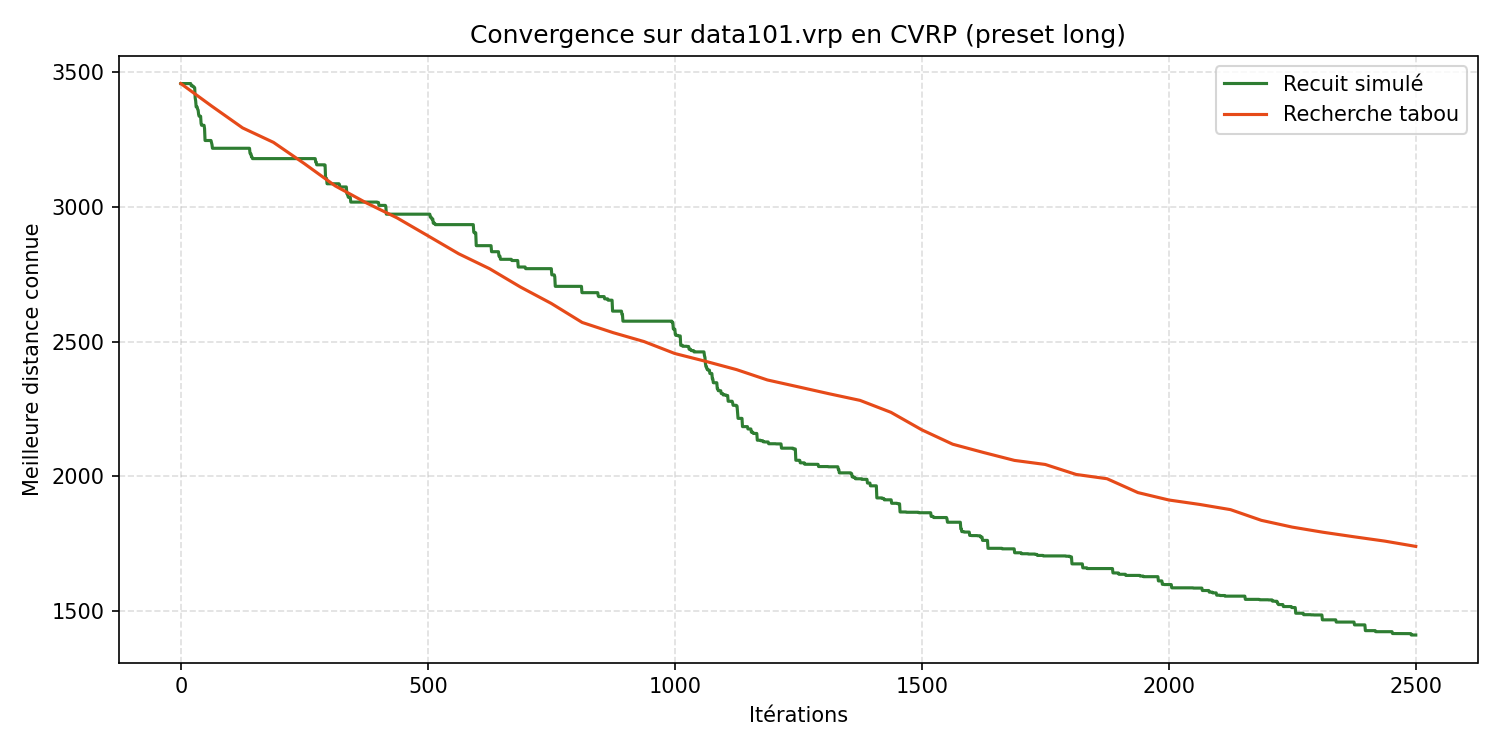
\includegraphics[width=\textwidth]{figures/convergence_data101_cvrp.png}
    \caption{Évolution de la distance (convergence) sur \texttt{data101.vrp} en CVRP.}
\end{figure}

Comme montré sur la figure précédente, le recuit simulé améliore très rapidement la solution dès les premières centaines d'itérations, puis continue à progresser plus finement. La recherche tabou, évaluée sur un nombre d'itérations beaucoup plus faible mais avec une exploration plus structurée à chaque étape, améliore elle aussi la solution initiale, mais converge ici vers un palier plus élevé. Cette figure confirme donc visuellement l'écart de qualité déjà mis en évidence dans les tableaux, tout en montrant que les deux méthodes ne parcourent pas l'espace des solutions de la même manière.

\subsection{Courbe de convergence en VRPTW}
Une seconde courbe de convergence est ajoutée dans le cadre du vrai problème avec fenêtres de temps, sur l'instance \texttt{data1201.vrp}. Cette figure est importante car elle permet d'observer le comportement des deux méthodes lorsque l'espace faisable est fortement restreint par les contraintes temporelles.

\begin{figure}[H]
    \centering
    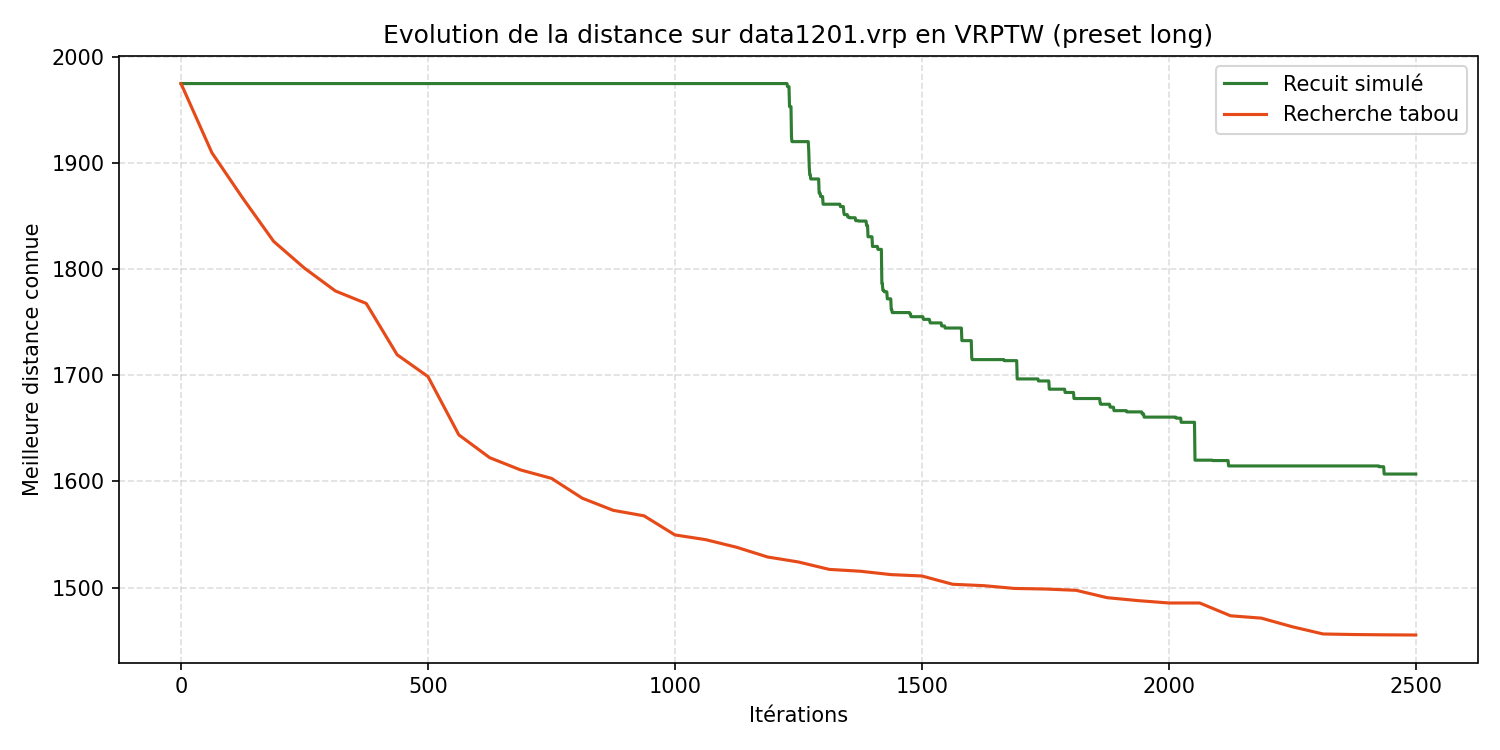
\includegraphics[width=\textwidth]{figures/convergence_data1201_vrptw.png}
    \caption{Évolution de la distance (convergence) sur \texttt{data1201.vrp} en VRPTW.}
\end{figure}

Comme montré sur cette figure, le recuit simulé améliore régulièrement la solution initiale, mais la recherche tabou finit ici par descendre plus bas. Cette observation est cohérente avec les résultats moyens de la campagne longue VRPTW : lorsque les contraintes temporelles resserrent fortement l'espace faisable, une exploration plus structurée peut devenir plus avantageuse qu'une exploration légère mais très fréquente.

\subsection{Synthèse de la première campagne longue}
À l'issue de cette première campagne longue menée sur l'ensemble des familles d'instances disponibles, une tendance forte se dégage :
\begin{itemize}
    \item le recuit simulé améliore systématiquement et fortement les solutions initiales ;
    \item la recherche tabou améliore également nettement les solutions après recalibrage, mais reste globalement en retrait par rapport au recuit simulé dans la version capacitaire ;
    \item le coût de calcul du recuit simulé reste faible sur toutes les instances testées ;
    \item le coût de calcul de la recherche tabou reste raisonnable, généralement entre \(4\) et \(17\) secondes par bloc de cinq répétitions.
\end{itemize}

Le tableau suivant résume les valeurs moyennes observées sur l'ensemble de cette première campagne longue.

\begin{center}
\begin{tabular}{lcccccc}
\toprule
Instance & \(k\) & Init. moy. & RS moy. & Tabou moy. & Temps RS (s) & Temps tabou (s) \\
\midrule
data101.vrp  & 8 & 3655.35 & 1266.78 & 1339.08 & 1.26  &  5.05 \\
data102.vrp  & 8 & 3537.80 & 1292.26 & 1309.82 & 1.11  &  4.57 \\
data1101.vrp & 9 & 4718.01 & 1634.58 & 1686.47 & 2.07  &  8.33 \\
data1102.vrp & 9 & 4675.37 & 1611.01 & 1720.14 & 2.06  &  8.41 \\
data111.vrp  & 8 & 3519.79 & 1250.95 & 1312.29 & 1.19  &  4.84 \\
data112.vrp  & 8 & 3542.86 & 1245.11 & 1305.22 & 1.13  &  4.55 \\
data1201.vrp & 2 & 4613.08 & 1311.63 & 1301.29 & 0.66  &  2.68 \\
data1202.vrp & 2 & 4366.31 & 1327.29 & 1335.45 & 0.65  &  2.66 \\
data201.vrp  & 2 & 3580.75 & 1197.26 & 1163.18 & 0.62  &  2.36 \\
data202.vrp  & 2 & 3379.92 & 1151.47 & 1115.68 & 0.55  &  2.29 \\
\bottomrule
\end{tabular}
\end{center}

Dans la version capacitaire, le recuit simulé reste la meilleure méthode en qualité sur 7 instances sur 10. Les trois exceptions (\texttt{data1201.vrp}, \texttt{data201.vrp}, \texttt{data202.vrp}) correspondent aux instances à grande capacité ($Q=1000$, $k=2$) : avec seulement deux véhicules, l'espace combinatoire est plus réduit et la mémoire tabou permet d'explorer plus efficacement les quelques transitions non triviales. Sur les instances à capacité standard ($Q=200$), le recuit simulé domine clairement. La recherche tabou recalibrée reste néanmoins très compétitive sur l'ensemble du corpus avec des temps de calcul raisonnables (entre 2 et 9 secondes par bloc de cinq répétitions).

% --------------------------------------------------
\subsection{Campagne VRPTW en mode rapide}
\label{sec:vrptw_quick}
Après le premier test ciblé décrit en section~\ref{sec:det_vehicules}, nous avons lancé une campagne \texttt{quick} sur l'ensemble des instances avec fenêtres de temps activées. Pour chaque instance, la solution initiale provient de la construction déterministe par insertion.

\begin{center}
\begin{tabular}{lcccccc}
\toprule
Instance & \(k\) & Init. & RS & Tabou & Temps RS (s) & Temps tabou (s) \\
\midrule
data101.vrp  & 21 & 2127.09 & 1977.60 & 2037.80 & 3.37 & 2.88 \\
data102.vrp  & 18 & 1794.68 & 1794.63 & 1734.64 & 1.17 & 1.04 \\
data1101.vrp & 18 & 2184.86 & 2022.51 & 2085.13 & 1.87 & 1.47 \\
data1102.vrp & 16 & 2035.58 & 1843.53 & 1948.35 & 1.37 & 0.95 \\
data111.vrp  & 14 & 1601.37 & 1563.78 & 1518.05 & 1.15 & 0.78 \\
data112.vrp  & 12 & 1434.70 & 1369.71 & 1312.92 & 1.47 & 0.72 \\
data1201.vrp & 5  & 1748.48 & 1748.48 & 1647.93 & 0.72 & 0.49 \\
data1202.vrp & 4  & 1948.06 & 1868.26 & 1874.74 & 0.65 & 0.54 \\
data201.vrp  & 5  & 1636.58 & 1617.42 & 1570.00 & 0.83 & 0.66 \\
data202.vrp  & 5  & 1600.85 & 1600.85 & 1534.96 & 0.51 & 0.41 \\
\bottomrule
\end{tabular}
\end{center}

Cette première campagne rapide montre que la recherche tabou surpasse déjà le recuit simulé sur six instances sur dix en VRPTW, ce qui contraste avec le cas CVRP. L'explication algorithmique est directe : en VRPTW, le voisinage faisable est beaucoup plus restreint (section~\ref{sec:operateurs}), ce qui rend l'exploration aléatoire légère du recuit simulé moins efficace face à la recherche guidée de la tabou — celle-ci évalue plusieurs candidats par itération et retient le meilleur non tabou, tirant ainsi mieux parti d'un espace de solutions réduit.

\subsection{Campagne VRPTW en mode long}
Nous avons prolongé cette étude avec une campagne \texttt{long} complète sur les dix instances, avec cinq répétitions par instance.

\begin{center}
\begin{tabular}{lcccccc}
\toprule
Instance & \(k\) & Init. moy. & RS moy. & Tabou moy. & Temps RS (s) & Temps tabou (s) \\
\midrule
data101.vrp  & 21 & 2127.09 & 1706.28 & 1683.01 & 56.81 & 336.61 \\
data102.vrp  & 18 & 1794.68 & 1584.73 & 1488.40 & 17.78 & 88.36  \\
data1101.vrp & 18 & 2184.86 & 1740.38 & 1713.19 & 31.90 & 214.38$^*$ \\
data1102.vrp & 16 & 2029.10 & 1593.91 & 1532.88 & 20.07 & 127.15 \\
data111.vrp  & 14 & 1601.37 & 1238.83 & 1190.92 & 13.34 & 49.77  \\
data112.vrp  & 12 & 1434.70 & 1105.87 & 1060.79 & 16.25 & 68.33  \\
data1201.vrp & 5  & 2027.69 & 1544.00 & 1445.97 & 12.31 & 54.46  \\
data1202.vrp & 4  & 1904.74 & 1443.74 & 1360.69 & 10.53 & 44.16  \\
data201.vrp  & 5  & 1653.00 & 1378.63 & 1268.26 &  9.35 & 44.81  \\
data202.vrp  & 5  & 1498.84 & 1331.76 & 1156.67 &  5.18 & 21.02  \\
\bottomrule
\end{tabular}
\end{center}

\subsection{Analyse de la campagne VRPTW longue}
Les résultats ci-dessus correspondent à des moyennes sur cinq répétitions. Le temps tabou de \texttt{data1101.vrp} est marqué d'un astérisque : le run~3 a enregistré un temps de \(5899\) s dû à une suspension OS ; la valeur \(214\) s correspond à la moyenne des quatre autres runs.

\begin{itemize}
    \item La recherche tabou devient meilleure que le recuit simulé sur la totalité des dix instances en VRPTW — résultat rare en CVRP (3 instances sur 10, toutes à grande capacité, $Q=1000$, $k=2$).
    \item L'écart algorithmique est quantifiable : la tabou évalue jusqu'à \(60 \times 200 = 12\,000\) candidats par répétition contre \(3\,000\) pour le RS, et sélectionne à chaque itération le meilleur voisin non tabou. Dans un espace faisable restreint (section~\ref{sec:operateurs}), cette stratégie gloutonne structurée est plus efficace que l'acceptation aléatoire du RS.
    \item Le surcoût en temps est réel : jusqu'à \(337\) s par répétition sur \texttt{data101.vrp} pour la tabou contre \(57\) s pour le RS. Ce compromis qualité/temps est à peser selon le contexte applicatif.
    \item Les améliorations les plus marquées se trouvent sur les instances à capacité élevée (\texttt{data201.vrp} : $-110$ u.d., \texttt{data202.vrp} : $-175$ u.d.), où l'espace de solutions est plus large et la tabou peut explorer plus de bassins distincts.
\end{itemize}

\begin{figure}[H]
    \centering
    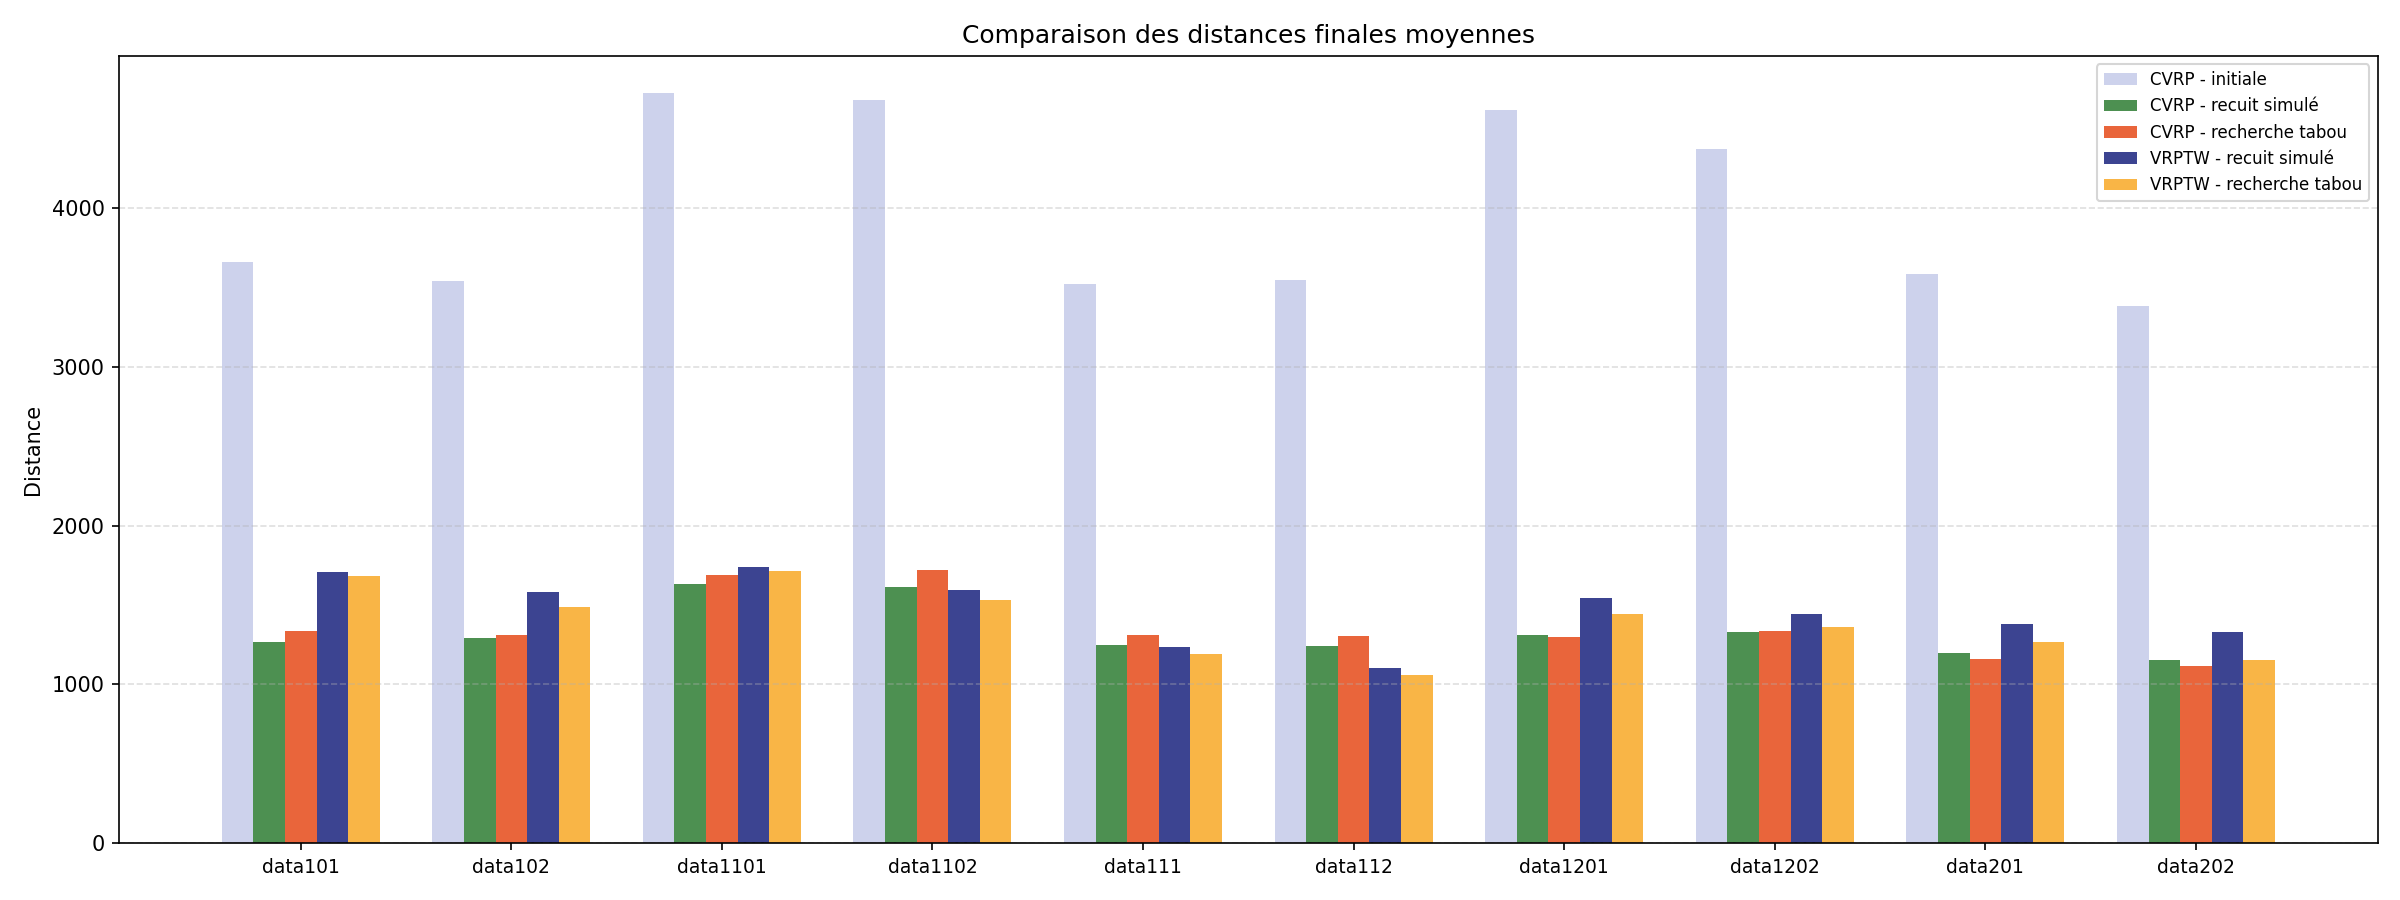
\includegraphics[width=\textwidth]{figures/comparison_distances.png}
    \caption{Comparaison des performances en distance finale sur les campagnes longues CVRP et VRPTW.}
\end{figure}

Comme montré sur cette figure, le recuit simulé est majoritaire en CVRP (7 instances sur 10), tandis que la recherche tabou domine nettement en VRPTW (10 instances sur 10). Cette lecture synthétique confirme que les performances relatives des métaheuristiques dépendent fortement de la structure faisable du problème.

\begin{figure}[H]
    \centering
    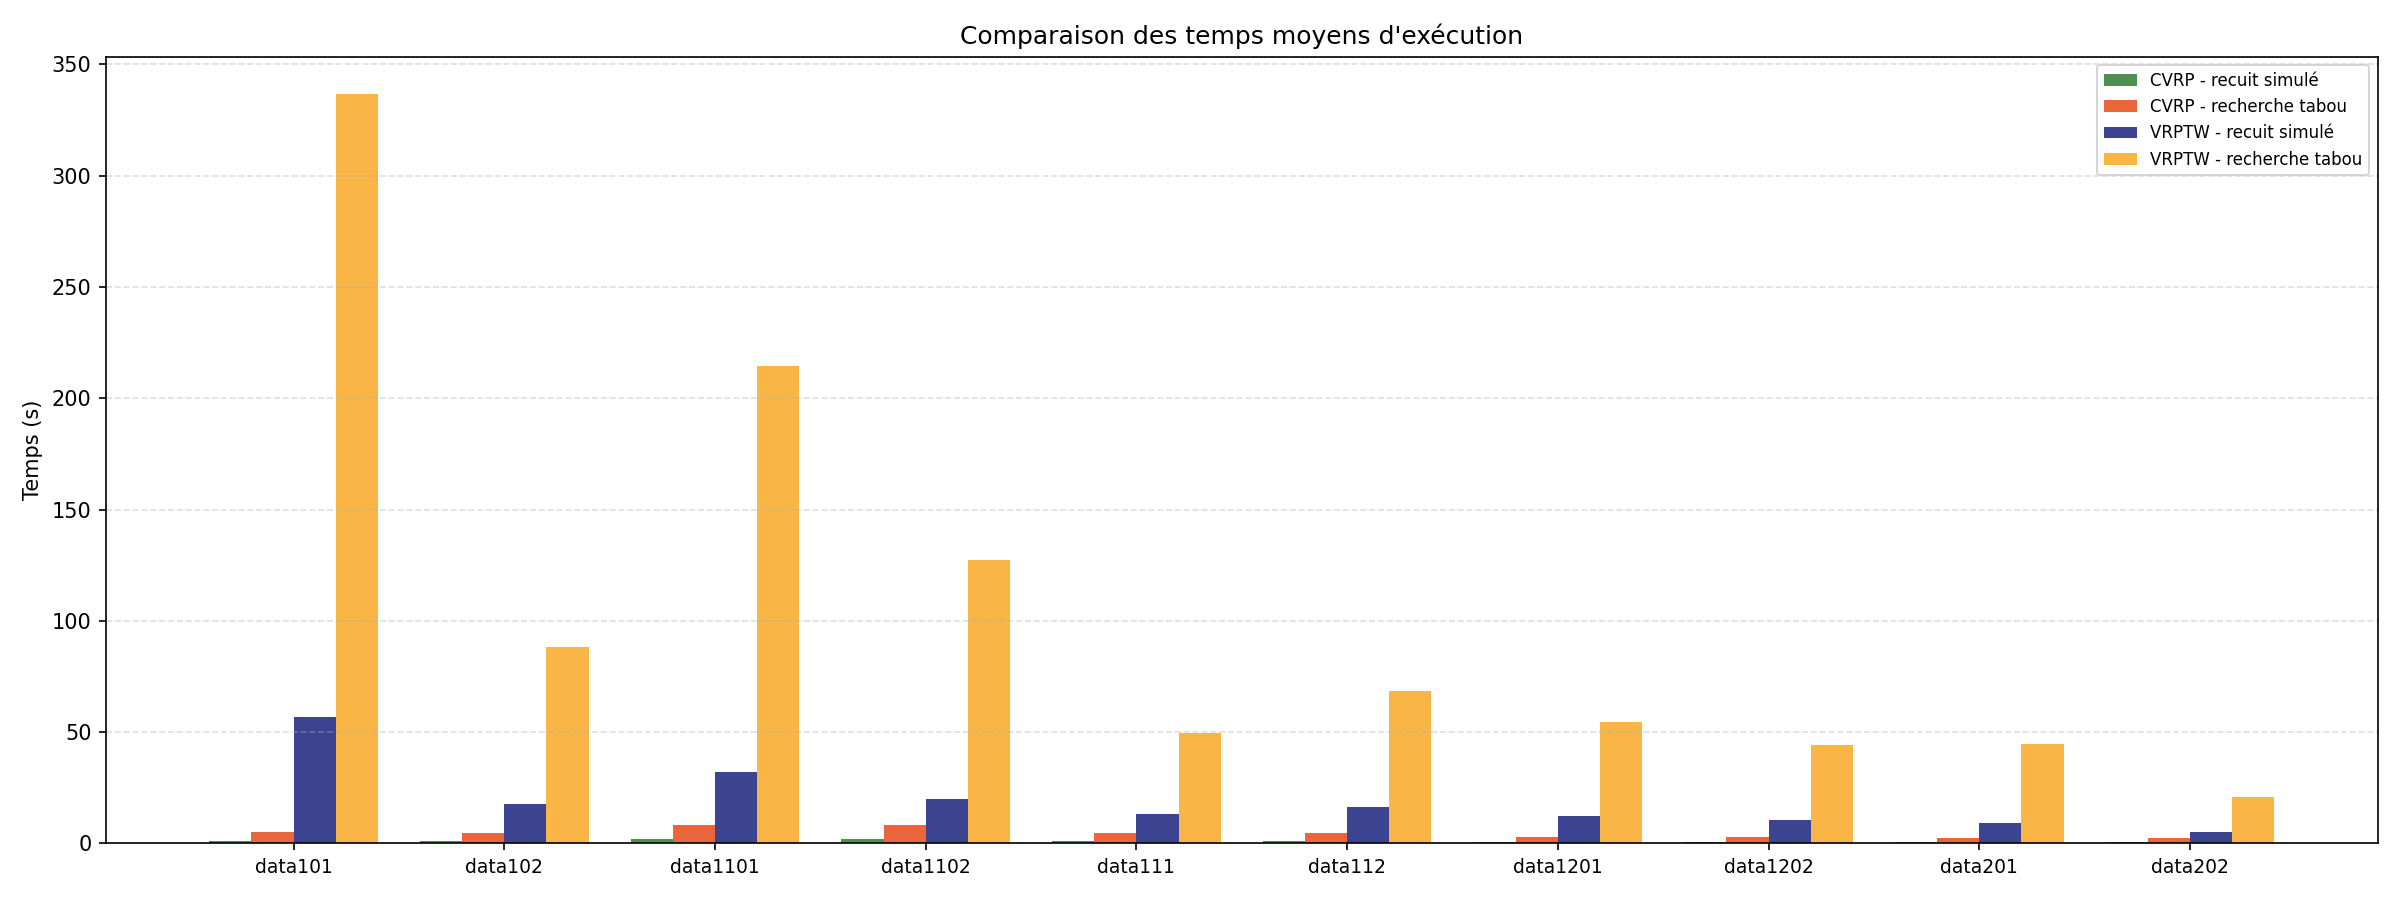
\includegraphics[width=\textwidth]{figures/comparison_times.png}
    \caption{Comparaison des performances en temps d'exécution sur les campagnes longues CVRP et VRPTW.}
\end{figure}

Comme montré sur cette figure, la recherche tabou reste plus coûteuse en temps que le recuit simulé, surtout en VRPTW. Cela implique qu'une meilleure qualité de solution ne s'obtient pas gratuitement : le compromis qualité/temps reste un élément central de l'analyse.

\subsection{Lecture synthétique du corpus et cas marquants}
Les campagnes finales \texttt{long} couvrent l'ensemble des dix instances du corpus, en CVRP comme en VRPTW. Nous disposons donc bien d'une base expérimentale complète pour dégager des tendances globales ; en revanche, toutes les instances n'ont pas besoin d'un commentaire détaillé dans le corps du rapport. Nous retenons ici trois cas particulièrement informatifs.

\texttt{data101.vrp} constitue d'abord le cas VRPTW le plus contraint de notre corpus, avec \(21\) véhicules trouvés par notre construction contre \(8\) en CVRP. Sur cette instance, la recherche tabou l'emporte avec une distance moyenne de \(1683.01\) contre \(1706.28\) pour le recuit simulé (moyenne sur cinq répétitions). L'écart de \(23\) unités (\({\approx}1{,}3\,\%\)) illustre que, même dans un espace faisable très contraint, la mémoire tabou permet d'exploiter plus finement les mouvements disponibles. Le coût en temps reste élevé pour la tabou (\({\approx}337\) s par répétition contre \({\approx}57\) s pour le recuit simulé), ce qui en fait la méthode à privilégier lorsque la qualité prime sur le temps de calcul. Cette instance joue donc le rôle de cas limite, utile pour comprendre le coût réel des contraintes temporelles les plus sévères.

\texttt{data1201.vrp} est ensuite un cas charnière, car il illustre très clairement le changement de régime entre CVRP et VRPTW. Sans fenêtres de temps, \(2\) véhicules suffisent ; la tabou passe devant légèrement (\(1301.29\) contre \(1311.63\) pour le RS). Avec fenêtres de temps, l'instance passe à \(5\) véhicules et l'avantage tabou se creuse nettement (\(1445.97\) contre \(1544.00\)). La visualisation des tournées montre concrètement cette fragmentation supplémentaire et rend visible l'effet structurel des contraintes temporelles.

Enfin, \texttt{data202.vrp} constitue un cas atypique très instructif en VRPTW. Sur la campagne longue finale, le recuit simulé améliore la solution initiale moyenne de \(1498.84\) à \(1331.76\), tandis que la recherche tabou descend à \(1156.67\). L'écart entre les deux méthodes est particulièrement marqué (\({\approx}175\) unités), ce qui suggère que certains bassins locaux nécessitent une mémoire explicite pour être quittés efficacement, et qu'une exploration plus structurée avec mémoire tabou peut alors devenir décisive.

Cette lecture par cas ne remplace donc pas l'analyse globale ; elle la complète. Le corpus complet sert à établir les tendances robustes, tandis que quelques instances ciblées permettent d'expliquer pourquoi ces tendances apparaissent.

\subsection{Exemple de visualisation de tournées}
La figure suivante illustre une visualisation explicite des tournées sur l'instance \texttt{data1201.vrp}. Afin de garder une figure lisible, nous représentons d'un côté une solution CVRP obtenue par recuit simulé et, de l'autre, une solution VRPTW obtenue par recherche tabou. Ces deux solutions sont effectivement reconstruites à partir du code final et d'une graine contrôlée.

Cette visualisation met en évidence un point important du projet : sur la même géométrie de clients, l'introduction des fenêtres de temps modifie fortement la structure des tournées et augmente le nombre de véhicules nécessaires. Dans le cas CVRP, la solution reste concentrée autour de \(2\) tournées, alors que la version VRPTW conduit ici à \(5\) tournées plus fragmentées.

\begin{figure}[H]
    \centering
    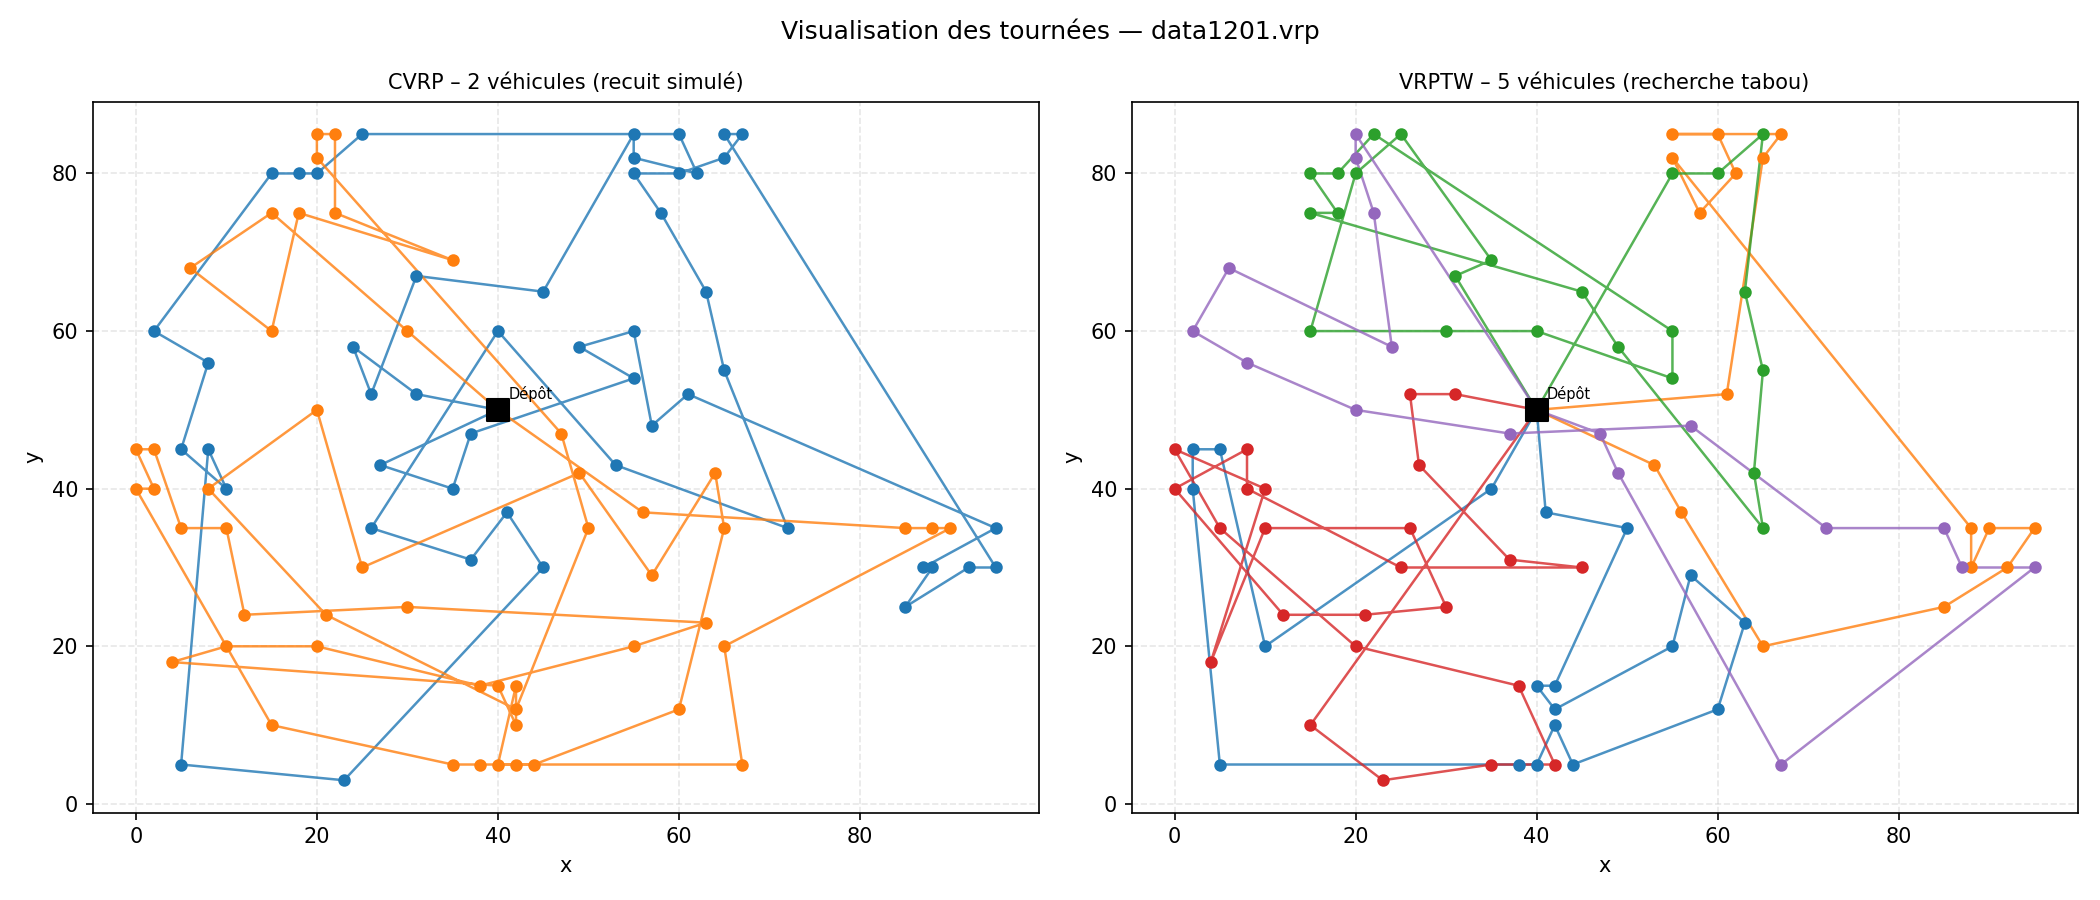
\includegraphics[width=\textwidth]{figures/routes_data1201_comparison.png}
    \caption{Visualisation comparative des tournées sur \texttt{data1201.vrp} : CVRP à gauche, VRPTW à droite.}
\end{figure}

% --------------------------------------------------
\section{Format des données}
% --------------------------------------------------

Les fichiers d'entrée sont des fichiers texte au format \texttt{.vrp}. Une instance contient :
\begin{itemize}
    \item le nom du fichier ;
    \item le nombre de dépôts ;
    \item le nombre de clients ;
    \item la capacité maximale d'un véhicule ;
    \item les informations sur le dépôt ;
    \item les informations sur chaque client.
\end{itemize}

Exemple de structure :
\begin{lstlisting}
NAME: data101.vrp
COMMENT:
TYPE: vrptw
COORDINATES: cartesian
NB_DEPOTS: 1
NB_CLIENTS: 100
MAX_QUANTITY: 200

DATA_DEPOTS [idName x y readyTime dueTime]:
d1 35 35 0 230

DATA_CLIENTS [idName x y readyTime dueTime demand service]:
c1 41 49 161 171 10 10
...
\end{lstlisting}

Chaque client est donc décrit par :
\begin{itemize}
    \item ses coordonnées \((x,y)\) ;
    \item sa fenêtre de temps \([readyTime, dueTime]\) ;
    \item sa demande ;
    \item sa durée de service.
\end{itemize}

% --------------------------------------------------
\section{Bonus : résolution exacte sur sous-instances}
% --------------------------------------------------

Le sujet proposait en bonus d'utiliser un package de programmation linéaire afin d'identifier à partir de quelle taille d'instance il devient difficile d'obtenir une solution exacte. Nous avons traité ce point avec OR-Tools, via le solveur linéaire SCIP, sur la version capacitaire du problème.

L'idée retenue est simple : partir d'une instance existante, construire des sous-instances contenant seulement les \(n\) premiers clients, puis résoudre exactement chacune de ces sous-instances avec une limite de temps fixée. Nous avons automatisé cette étude dans un module dédié, de façon à pouvoir relancer facilement les tests sur plusieurs tailles.

Pour cette première étude, nous sommes partis de \texttt{data101.vrp} et avons testé les tailles \(5\), \(10\), \(15\), \(20\), \(25\), \(30\), \(35\) et \(40\) clients, avec une limite de \(10\) secondes par sous-instance.

\begin{center}
\begin{tabular}{ccccc}
\toprule
Clients & \(k\) & Statut & Objectif & Temps (s) \\
\midrule
5  & 1 & OPTIMAL  & 119.48 & 0.03 \\
10 & 1 & OPTIMAL  & 173.04 & 0.01 \\
15 & 2 & OPTIMAL  & 248.91 & 0.74 \\
20 & 2 & OPTIMAL  & 280.13 & 0.46 \\
25 & 2 & OPTIMAL  & 335.27 & 5.08 \\
30 & 3 & FEASIBLE & 364.88 & 10.01 \\
35 & 3 & FEASIBLE & 444.35 & 10.01 \\
40 & 3 & FEASIBLE & 561.89 & 10.01 \\
\bottomrule
\end{tabular}
\end{center}

L'enseignement principal est net : dans notre configuration, le solveur exact reste très efficace jusqu'à \(25\) clients, mais commence à peiner dès \(30\) clients, où il atteint déjà la limite de temps sans certifier l'optimalité. Ce seuil ne constitue pas une frontière théorique universelle, mais il donne un ordre de grandeur concret sur le moment où une approche exacte devient sensiblement plus difficile à exploiter dans ce projet.

% --------------------------------------------------
\section{Limites et perspectives}
\label{sec:limites}
% --------------------------------------------------

Le travail réalisé permet de répondre à l'ensemble des points principaux du sujet, mais certaines limites doivent être signalées.
\begin{itemize}
    \item Dans le cas VRPTW, la génération aléatoire de solutions initiales a été nettement améliorée, mais elle reste moins robuste que dans la version purement capacitaire.
    \item La recherche tabou recalibrée obtient de très bons résultats sur la campagne finale VRPTW, mais son coût de calcul demeure plus élevé sur quelques instances difficiles, en particulier lorsque le nombre de véhicules imposé par les fenêtres de temps devient important.
    \item L'étude exacte avec OR-Tools a volontairement été limitée à des sous-instances de petite taille ; elle fournit donc un ordre de grandeur utile, mais pas une frontière générale de difficulté.
\end{itemize}

Ces limites ouvrent des perspectives naturelles : renforcer l'initialisation aléatoire en VRPTW, affiner les paramètres sur les cas les plus contraints, élargir l'étude exacte à d'autres familles de sous-instances.

\subsection{Discussion sur la validité des résultats}

\textbf{Significativité statistique.} Avec $n=5$ répétitions, l'erreur standard sur la moyenne est $\sigma/\sqrt{5} \approx 0{,}45\,\sigma$. Les différences inférieures à $1\,\%$ entre les deux méthodes — comme les $10$ unités d'écart sur \texttt{data1201.vrp} en CVRP ($\approx 0{,}8\,\%$) — sont dans l'ordre de grandeur de cette incertitude et ne permettent pas de conclure sur une supériorité structurelle. Les différences plus grandes ($>5\,\%$), notamment en VRPTW, sont en revanche robustes.

\textbf{Reproductibilité.} Un bug dans l'opérateur \texttt{or-opt(2)} a été détecté et corrigé en cours de projet (skip invalide dans les mouvements intra-route). Ce bug modifiait la séquence aléatoire et faussait les résultats CVRP d'environ $3$--$5\,\%$. Toutes les valeurs publiées dans ce rapport ont été produites avec la version corrigée du code. Les résultats VRPTW sont peu affectés car \texttt{or-opt(2)} représente environ $1\,\%$ du voisinage faisable en VRPTW.

\textbf{Comparaison qualitative avec la littérature.} Les instances de ce corpus s'inscrivent dans la famille des problèmes de routage à $100$ clients avec fenêtres de temps, de structure analogue aux benchmarks Solomon (1987). Pour des instances de type R1xx (contraintes temporelles moyennement serrées, $k\approx 19$--$21$), la littérature spécialisée cite des solutions de référence autour de $1\,600$--$1\,700$ unités de distance ; nos meilleures valeurs tabou ($1\,683$ sur \texttt{data101.vrp}, $1\,488$ sur \texttt{data102.vrp}) se situent dans cet ordre de grandeur. Pour des instances de type C1xx (clients groupés géographiquement, $k$ faible), les meilleures solutions connues sont nettement plus basses : un écart plus important est donc attendu sur les instances à grande capacité. Cette comparaison reste indicative, car nos instances ne sont pas les benchmarks Solomon standardisés et n'ont pas été soumises à des algorithmes spécialisés.

% --------------------------------------------------
\section{Conclusion}
% --------------------------------------------------

Ce projet aboutit à une chaîne complète de résolution du problème, de la modélisation aux campagnes expérimentales, en passant par la construction de solutions initiales, les voisinages et deux métaheuristiques distinctes.

Trois résultats ressortent nettement. D'abord, sur le corpus CVRP étudié, notre procédure heuristique a trouvé une solution faisable dès la borne inférieure capacitaire $LB$ pour chaque instance ; dans ce cas précis, la borne de capacité certifie donc le nombre minimal de véhicules. Ensuite, l'introduction des fenêtres de temps augmente fortement le nombre de véhicules trouvé par construction et resserre l'espace des solutions faisables. Enfin, les performances relatives des métaheuristiques dépendent de cette structure : le recuit simulé constitue le meilleur compromis en CVRP sur 7 instances sur 10, avec la tabou devant sur les trois instances à grande capacité ($Q=1000$, $k=2$) ; en VRPTW, la recherche tabou devient systématiquement meilleure sur la totalité du corpus dans la campagne longue finale.

\subsection{Comment nous cherchons l'optimum}

Notre stratégie de résolution repose sur une décomposition en trois couches.

\textbf{Couche 1 — Construction.} Nous déterminons un nombre de véhicules $k$ par une heuristique de construction, en incrémentant depuis la borne inférieure capacitaire $LB$ jusqu'à obtenir une solution faisable. En CVRP, le $k$ trouvé coïncide avec $LB$ sur notre corpus et est donc minimal au sens capacitaire. En VRPTW, une construction déterministe par insertion prend le relais lorsque la construction aléatoire échoue ; le $k$ obtenu est le premier trouvé faisable par notre méthode, pas une preuve exacte de minimalité. Cette solution initiale fournit un point de départ réaliste mais sous-optimal.

\textbf{Couche 2 — Voisinage local.} À partir de la solution initiale, nous explorons un voisinage défini par cinq opérateurs : \textit{relocate} (déplacement d'un client vers une autre position ou tournée), \textit{swap} (échange de deux clients quelle que soit leur tournée), \textit{2-opt} intra-route (inversion d'un segment dans une même tournée), \textit{Or-opt(2)} (déplacement d'une paire de clients consécutifs) et \textit{2-opt$^*$} (échange des suffixes de deux tournées distinctes). Chaque candidat est validé par le module \texttt{evaluate.py} avant d'être proposé à la métaheuristique, garantissant que seules des solutions faisables sont examinées.

\textbf{Couche 3 — Métaheuristiques.} Les deux métaheuristiques pilotent l'exploration à l'échelle globale :
\begin{itemize}
    \item le recuit simulé accepte des mouvements dégradants avec probabilité $\exp(-\Delta/T)$, ce qui permet d'échapper aux minima locaux ; la température $T$ décroît géométriquement selon le facteur de refroidissement $\alpha = 0{,}997$, réduisant progressivement l'exploration au profit de l'exploitation ;
    \item la recherche tabou interdit les solutions récemment visitées (mémoire FIFO de taille \textit{tenure} = 20) et sélectionne toujours le meilleur voisin non tabou, avec un critère d'aspiration pour ne pas bloquer une amélioration globale.
\end{itemize}

Ces conclusions reposent sur l'ensemble du corpus final et non sur quelques exemples isolés ; les études de cas détaillées servent seulement à interpréter les comportements les plus marquants.

\subsection{Synthèse globale des résultats}

Le tableau suivant résume les tendances principales issues des campagnes longues (5 répétitions, preset \texttt{long}).

\begin{center}
\begin{tabular}{lcccc}
\toprule
 & \multicolumn{2}{c}{CVRP (10 instances)} & \multicolumn{2}{c}{VRPTW (10 instances)} \\
\cmidrule(lr){2-3}\cmidrule(lr){4-5}
 & RS & Tabou & RS & Tabou \\
\midrule
Instances gagnées & 7/10 & 3/10 & 0/10 & 10/10 \\
Amélioration moy. / init. & ${\approx}65\,\%$ & ${\approx}63\,\%$ & ${\approx}56\,\%$ & ${\approx}61\,\%$ \\
Temps moyen par run & ${\approx}1{,}2$ s & ${\approx}4{,}8$ s & ${\approx}19$ s & ${\approx}73$ s \\
\bottomrule
\end{tabular}
\end{center}

En CVRP, les deux méthodes améliorent les solutions initiales dans des proportions proches ($\approx63$--$65\,\%$) ; le recuit simulé domine légèrement sur les instances à capacité modérée ($Q=200$). En VRPTW, la recherche tabou tire parti de façon systématique de son exploration structurée dans un espace faisable restreint, au prix d'un temps de calcul environ $4\times$ supérieur. Ce rapport qualité/temps est le critère pratique principal pour choisir entre les deux approches.

\subsection{Améliorations envisageables}

Plusieurs directions permettraient encore d'améliorer la qualité des résultats.

\textbf{Heuristique de construction plus performante.} L'algorithme Solomon I1, qui insère les clients un par un en maximisant un critère combinant économie de distance et urgence temporelle, fournirait des solutions initiales de meilleure qualité que notre greedy géographique, notamment en VRPTW fortement contraint. Une meilleure initialisation réduirait également la dépendance aux répétitions multiples.

\textbf{Refroidissement adaptatif.} Plutôt qu'un facteur de refroidissement géométrique fixe ($\alpha = 0{,}997$), un refroidissement adaptatif qui ajuste la température en fonction du taux d'acceptation des dernières itérations permettrait de mieux calibrer l'exploration sans réglage manuel des paramètres.

\textbf{Séquence d'opérateurs guidée.} Plutôt qu'un tirage uniforme parmi les cinq opérateurs, une stratégie adaptative qui favorise les opérateurs ayant récemment produit des améliorations (bandit multi-bras) exploiterait plus efficacement le budget de calcul disponible.

\subsection{Critique du protocole expérimental}

\textbf{Diversité des solutions initiales en VRPTW.} En VRPTW fortement contraint, la construction aléatoire échoue presque systématiquement (taux d'échec supérieur à $97\,\%$ sur \texttt{data101.vrp}). Notre filet de sécurité — la construction déterministe — retourne alors toujours la même solution initiale pour toutes les répétitions. Conséquence directe : les répétitions démarrent du même point et la variabilité observée ne reflète que les fluctuations stochastiques intra-run, et non une vraie diversité inter-runs. Une initialisation basée sur plusieurs heuristiques déterministes différentes (greedy géographique, greedy temporel, Solomon I1) corrigerait ce biais.

\textbf{Nombre de répétitions et significativité statistique.} Notre préréglage \texttt{long} utilise cinq répétitions. L'erreur standard sur la moyenne est $\sigma/\sqrt{n}$ : avec $n = 5$ on obtient $\sigma/2{,}24$, contre $\sigma/3{,}16$ avec $n = 10$. Augmenter à dix répétitions diviserait l'incertitude par $1{,}41$ supplémentaire, au prix d'un facteur $\times 2$ sur le temps de calcul. C'est un compromis raisonnable pour une étude définitive.

\textbf{Mémoire tabou par signature globale.} Nous encodons chaque solution par sa signature complète, c'est-à-dire le tuple ordonné des routes et des clients. Cette représentation est simple et sans collision volontaire dans notre encodage, mais elle reste moins informative qu'une mémoire fondée directement sur les mouvements. Une mémoire tabou basée sur les mouvements eux-mêmes (paire de clients concernés, type d'opérateur) serait plus précise pour contrôler les retours arrière et permettrait de raisonner plus finement sur la diversification.

\end{document}
